\documentclass[12pt, a4paper, french, openright]{report}
% version reliée
% \documentclass[11pt, a4paper, french, openright, twoside]{report}
\usepackage{svg}
\usepackage{lipsum}
\usepackage[french]{babel}
\selectlanguage{french}
\usepackage[T1]{fontenc}
\usepackage[utf8]{inputenc}
\usepackage{lmodern,textcomp}
\usepackage[
    left = \flqq,%
    right = \frqq,%
    leftsub = \flqq,%
    rightsub = \frqq%
]{dirtytalk}

\usepackage{csquotes}
\usepackage{hyperref}

\usepackage{graphicx}
\usepackage{caption}
\usepackage{setspace}
\usepackage[footnote]{acronym}
\usepackage{titling}

\usepackage[toc,page]{appendix}
\renewcommand{\appendixpagename}{Annexes}
\renewcommand{\appendixtocname}{Annexes}

\usepackage[backend=biber, style=alphabetic]{biblatex}
\bibliography{bibliography}

\newcommand{\HRule}{\rule{\linewidth}{0.5mm}}
\renewcommand{\thefootnote}{\arabic{footnote}}

\usepackage{fancyhdr}
\pagestyle{fancy}
\fancyhf{}

\renewcommand{\chaptermark}[1]{\markboth{\bsc{\chaptername~\thechapter{} :} #1}{}}
\renewcommand{\sectionmark}[1]{\markright{\thesection{} \ #1}}
\renewcommand{\headrulewidth}{0pt}
%\lhead[\textsl{\leftmark}]{\textsl{\rightmark}}
\chead[\textsl{\rightmark}]{\textsl{\leftmark}}
\cfoot[\thepage]{\thepage}
\setlength{\headheight}{15pt}

\let\headruleORIG\headrule
\renewcommand{\headrule}{\color{black} \headruleORIG}
\renewcommand{\headrulewidth}{1.0pt}
\usepackage{colortbl}
\arrayrulecolor{black}

\renewcommand{\footrulewidth}{0.4pt}% 

\usepackage{sectsty}
\usepackage{lipsum}% just to generate some text


\chaptertitlefont{\centering \MakeUppercase}




\title{Interprétabilité et explicabilité des modèles boites noires}

\author{Damien JAIME}


\begin{document}

\begin{titlepage}
\begin{center}

% Upper part of the page. The '~' is needed because only works if a paragraph has started.
\setlength{\parindent}{0pt}

\includesvg[width=\textwidth]{upnsvg}~\\[1cm]

%
\includegraphics[width=1\textwidth]{./upn}~\\[1cm]

\textsc{\Huge Master 2 MIAGE}\\[0.5cm]

\vspace{5mm}

\textsc{\huge \bfseries  Mémoire de fin d'études}\\[1.5cm]



% Title
\HRule

{\huge \bfseries \thetitle \\[0.4cm] }


\HRule

\vspace{5mm}

% Author and supervisor
\begin{minipage}{0.4\textwidth}
\begin{flushleft} \large
\emph{\textbf{Auteur:}}\\
Damien \textsc{\textbf{JAIME}}
\end{flushleft}
\end{minipage}
\begin{minipage}{0.4\textwidth}
\begin{flushright} \large
\emph{\textbf{Tuteur :}} \\
Emanuel \textsc{\textbf{HYON}}
\end{flushright}
\end{minipage}

\vfill

% Bottom of the page
{\huge \bfseries Promotion 2019-2020}

\end{center}
\end{titlepage}

%page blanche
\newpage
~
%ne pas numéroter cette page
\thispagestyle{empty}
\newpage

%ne pas numéroter cette page
\thispagestyle{empty}
\begin{center}
\subsection*{Remerciements}
\end{center}

\hskip7mm

\begin{spacing}{1.3}
Ce mémoire symbolise la fin de cinq années d'études dans le supérieur. Je tiens tout d'abord à remercier tous les professeurs et les intervenants que j'ai rencontré, qui m'ont instruit et permis d'évoluer.

\vspace{5mm}

Je tiens tout particulièrement à remercier mon tuteur pour ce mémoire, monsieur Emmanuel HYON, pour m'avoir orienté, conseillé, mis a disposition de nombreuses ressources et pistes de réflexions.

\vspace{5mm}

Je remercie aussi monsieur Pascal Poizat, mon responsable de Master, pour son encadrement et ses conseils dans la réalisation de ce mémoire.

\vspace{5mm}


\end{spacing}

%page blanche
\newpage
~

~
\thispagestyle{empty}

\setcounter{tocdepth}{1}
\tableofcontents
\thispagestyle{empty}
\setcounter{page}{0}
%ne pas numéroter le sommaire

\newpage
~
\thispagestyle{empty}
%recommencer la numérotation des pages à "1"
\setcounter{page}{0}
\newpage

\chapter*{Introduction}
\addcontentsline{toc}{chapter}{Introduction}
\markboth{Introduction}{Introduction}
\label{chap:introduction}
\vspace{5mm}
\paragraph{}Nous sommes au quotidien en contact avec une multitude de boites noires, c’est-à-dire un système cachant sa logique interne à l’utilisateur. L’utilisateur ne pouvant pas savoir ce qu’il se passe dans le système, de nombreuses questions se posent. Notamment sur la confiance à accorder en ces systèmes, mais aussi d’un point de vue éthique particulièrement sur les questions de discrimination et de protection de la vie privée de l’utilisateur.

\paragraph{}Avec l’avènement de l’intelligence artificielle dans l’aide à la prise de décision, la problématique de compréhension de ces systèmes est devenu un des enjeux majeurs de notre génération. En effet, comment peut-on être assuré que notre modèle est réellement fiable ? Notre modèle a-t-il involontairement hérité de biais présent dans ses jeux de données d'entraînement ? Quel degré de compréhension est-il nécessaire de fournir et pour quelle complexité ?\\
Ces questions sont très importantes dans le domaine médical par exemple où un faux négatif peut être très problématique, car à la différence des faux positifs il n'y a pas de vérification postérieure effectué par l'humain. Par ailleurs, nombreux sont les cas où une intelligence artificielle a hérité de biais involontaire présent dans ses jeux de données d'entraînement engendrant différents types de discriminations. Comme par exemple l'intelligence artificielle de recrutement de l'entreprise Amazon qui rejetait automatiquement les CVs contenant le mot "femme"\cite{amazonAi}.

\paragraph{}Depuis 2016, en Europe, le Règlement Général de l'Union européenne sur la Protection des Données (RGPD) impose un droit à l'explication des décisions algorithmiques prises au sujet d'un utilisateur \cite{RGPDexplanRight}. Or les raisons des décisions de ces algorithmes étant très abstraites même pour la personne l'aillant créée, un problème se pose et les utilisateurs ne peuvent pas réellement utiliser ce droit à l'explication.

\paragraph{}En plus des questions d'éthique et de protection des utilisateurs, expliquer ces boites noires serait d'une très grande aide pour les entreprises afin de créer des produits plus sûr, plus efficacement et les aider à mieux gérer les problèmes de responsabilité.\par
Pour toutes ces raisons, fournir une explication à un système de décision type boite noire est un sujet de parfaite actualité suscitant de nombreuses attentes et tables rondes. Le "Gartner hype cycle for Emerging Technologies" de 2019 place ce sujet (Explainable AI) dans le pic des attentes et suppose une maturité dans les cinq à dix ans.

\paragraph{}L’objectif de ce mémoire est donc de comprendre comment un système boite noire et plus spécifiquement comment une intelligence artificielle est amenée à prendre une décision. Pour cela, nous allons analyser les différentes méthodes existantes dans la littérature et les appliquer à plusieurs cas concrets. Afin de savoir si expliquer ces systèmes boite noire nous permettrait de résoudre les problèmes auxquels ils sont confrontés et pour lesquels ils sont tant critiqués. Les applications porteront donc sur les questions d'éthique, de fiabilité et de performance.\\

\paragraph{}Le reste de ce mémoire sera organisé en plusieurs parties. Tout d'abord, nous commencerons par contextualiser afin de bien comprendre les différentes problématiques et dérives existantes. Nous enchaînerons par la suite avec un état de l'art divisé en deux parties : la première sera axée sur des définitions et présentations d'éléments conceptuels portant sur l'interprétabilité et de l'explicabilité, tandis que la seconde traitera des différentes méthodes et outils existant afin d'expliquer différents types de boite noire. La suite consistera donc à appliquer ces méthodes afin de d'évaluer leurs capacités à rendre un système de décision compréhensible par l'homme et de voir si ces explications permettent de palier aux problématiques décrites précédemment.



\chapter{Contexte : un besoin d'explicabilité}
Expliquer les modèles de décisions boites noires est un besoin se faisant de plus en plus ressentir et suscitant de nombreux débats et tables rondes dans la communauté scientifique. Les entreprises recherchent avant toute chose la performance et ce au détriment de la transparence des algorithmes utilisés. En effet dans le domaine du machine learning il existe une multitude d'algorithmes pouvant être utilisés afin de fournir une prédiction, mais il existe une corrélation non négligeable entre les performances et la transparence de notre modèle comme le montre la figure \ref{performanceAndInterpretabilite}. En général, plus notre modèle est performant, plus il est difficile à comprendre.\par

\begin{figure}[h]
\centering
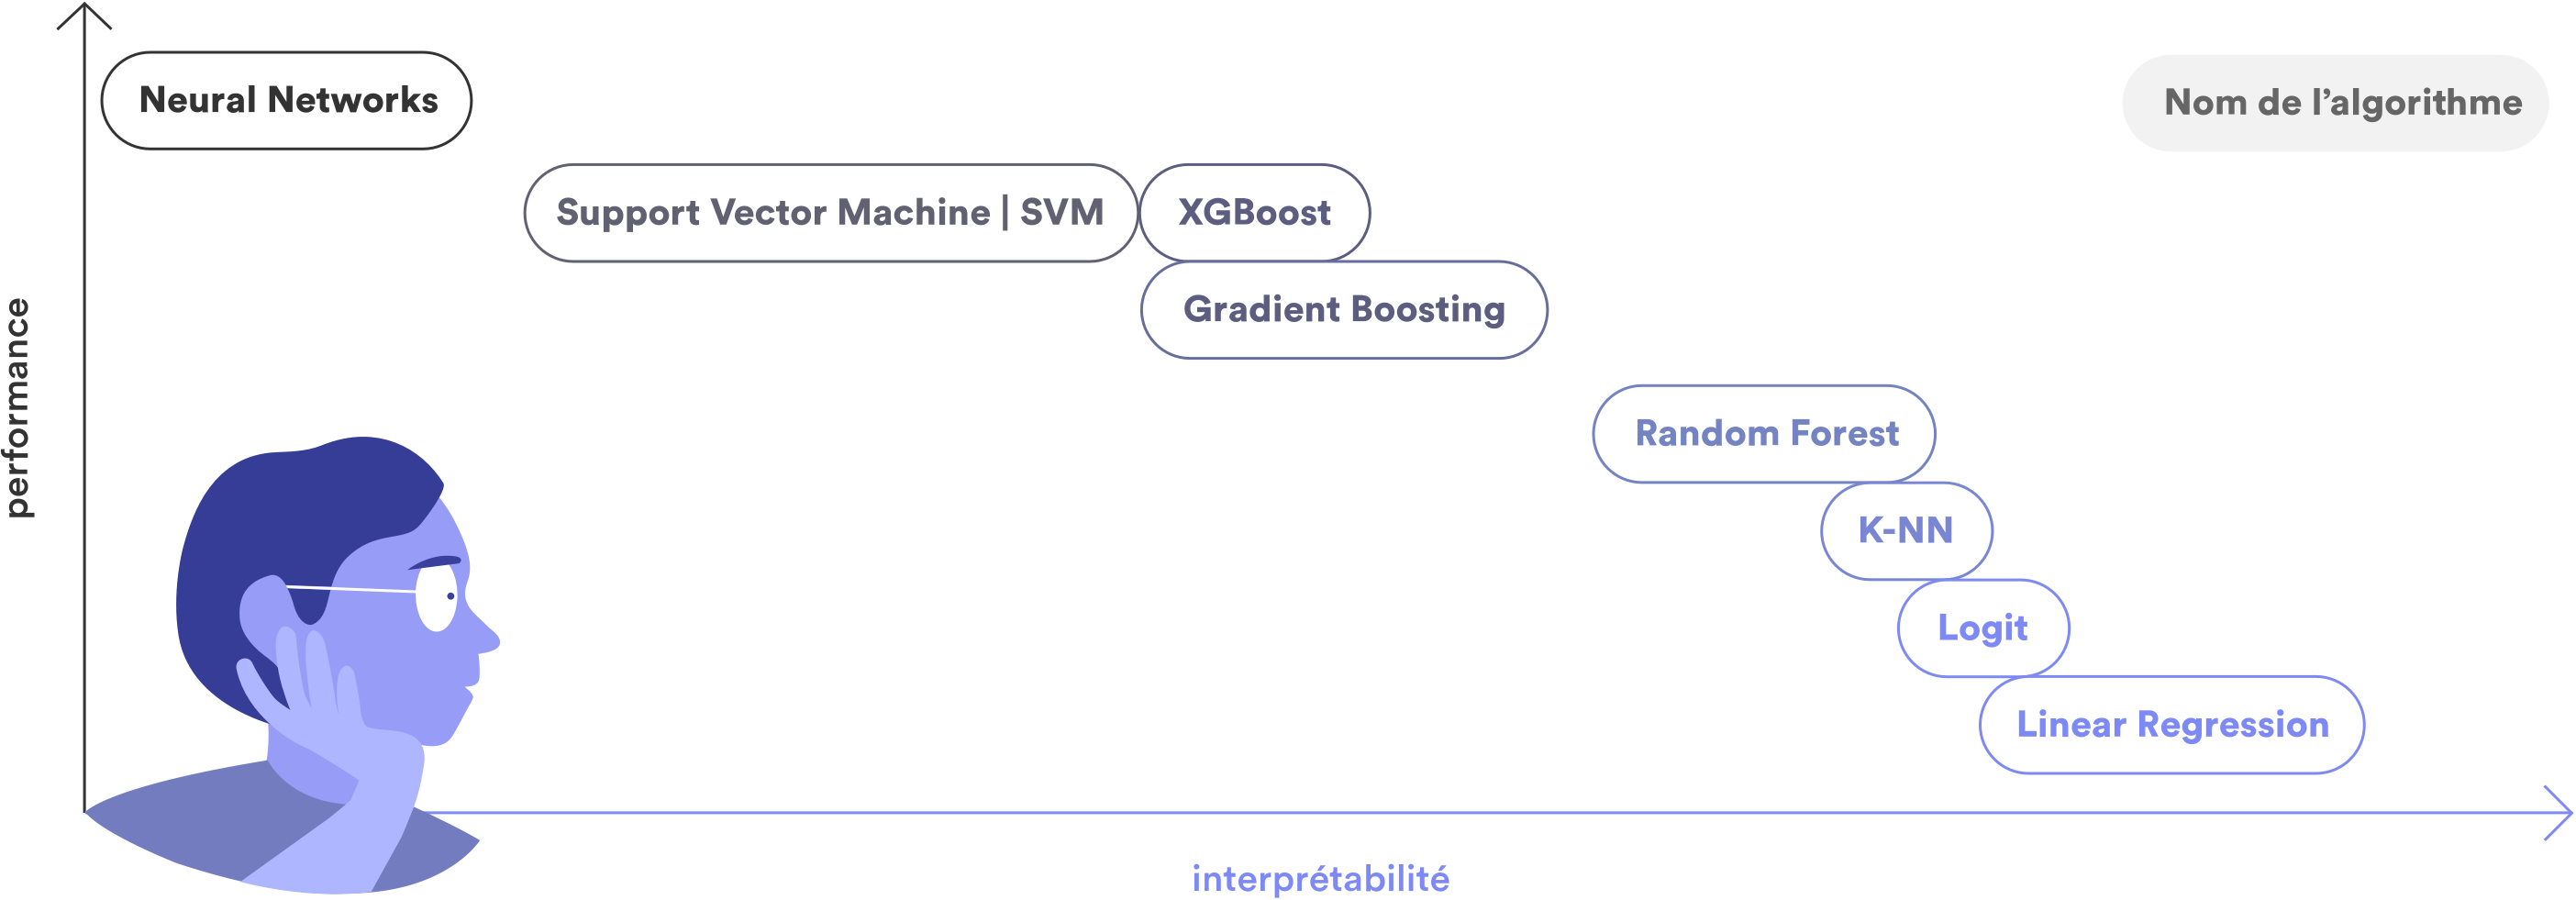
\includegraphics[scale=0.15]{src_img/performanceAndInterpretabilite.png}
\caption{Lien entre la performance et l'interprétabilité d'un algorithme de machine learning. \textit{Source \cite{hippocrate}}}
\label{performanceAndInterpretabilite}
\end{figure}

À l'heure actuelle, le réseau de neurones artificiel fait partie des algorithmes les plus performante et est le plus couramment utilisée.
La non-explicabilité de ces modèles posent des problèmes de fiabilité, d'éthique et de responsabilité. Ce floue accentue aussi la méfiance et la peur des personnes envers l'intelligence artificielle, et entraîne un problème de compréhension entre les Data Scientist et les expert métier qui en plus de ne pas comprendre comment fonctionne le modèle ne comprennent pas non plus les raisons de son résultat. Aussi, expliquer ces modèles permettrai d'améliorer notre conformité à la loi (notamment vis-à-vis de la RGPD évoqué en introduction) ainsi que d'augmenter les performances de nos modèles. Cette nouvelle problématique présente donc de nombreux enjeux de tailles.\par
Ce besoins d'explicabilité se fait tellement ressentir qu'il devient un enjeu de taille même pour les plus hautes instances de l'état. Ainsi, en 2017, le Premier Ministre Français Édouard Philippe confit au mathématicien et député Cédric Villani une mission parlementaire d’information sur la stratégie française et européenne à adopter en matière d'intelligence artificielle. Communément appelé "Rapport Villani" \cite{rapportVillani}, il consacre toute une partie sur les questions d'éthique et arrive au constat suivant : le principal problème vient du fait que l'IA est une boîte noire. L'explicabilité de l'IA est un aspect fondamental de ce rapport et Villani donne des pistes pour améliorer ce domaine :
\begin{itemize}
    \item \textbf{L’audit des IA} : Villani propose \textit{"La constitution d’un corps d’experts dotés des compétences requises semble nécessaire pour procéder à des audits d’algorithmes et de bases de données sur pièce, et procéder à des tests par tout moyen requis."} L'idée est donc d'effectuer des contrôles dans les entreprises afin de palier à toutes dérives.
    \item \textbf{L’évaluation citoyenne des IA} : L'idée est la même que la précédente, mais appuis le fait que le contrôle, en plus d'être mis en place par un organe public, doit aussi provenir de la société civile.
    \item \textbf{Soutenir la recherche sur l’explicabilité} : L'IA et son explicabilité étant des disciplines récentes, le gouvernement se doit d'investir dans la recherche et de favoriser une collaboration étroite entre pouvoirs publics, laboratoires de recherche et industriels.
\end{itemize}

\section{Impact social de l'intelligence artificielle}
Dans son livre "Weapons of Math Destruction" \cite{mathDestruction} l'américaine Cathy O'Neil qui a une formation en mathématiques, a été trader, puis data scientist dénonce l'impact social engendré par l'utilisation permanente des modèles prédictifs dans nos vies. Le sous-titre de ce livre, qui en résume le propos, est "Comment le big-date augmente les inégalités et menace la démocratie". Pour commencer, Cathy O'Neil souligne le fait qu'un modèle prédictif ne peut pas couvrir la complexité du vrai monde, que les modèles se basent sur des comportements passés et classent les individus en tribus de façon arbitraire alors que la réalité est beaucoup plus complexe. De ce fait, le risque d'erreur est important et les probabilités ne reflètent pas forcément la réalité. Un autre problème est que les jeux de données utilisés ne sont pas nécessairement fiables ou adaptées au modèle et que ces modèles reflètent les choix subjectifs de leurs concepteurs. Le dernier problème majeur soulevé est que ces modèles sont opaques et qu'il n'est pas possible, contrairement au jugement humain, de faire appel en cas de désaccord. En autre, il est possible de camoufler des choix subjectifs (jugements raciaux ou discriminatoires par exemple) en créent un modèle émettant les prédictions allant dans le sens voulu afin de dédouaner la responsabilité sur le modèle. \par
L'intelligence artificielle aurai donc pour effet de renforcer le déterminisme social et ainsi d'augmenter les inégalités. Là encore, expliquer ces décisions permettrai de prévenir les dérives et rendre l'explication obligatoire, dans certains cas, permettrai de remettre la responsabilité sur les concepteurs de ces modèles.

\section{L'éthique}
De nombreux cas très exposés dans les médias nous montrent que l'incompréhension à l'égard de l'IA peut amener à des problèmes du point de vue éthique. La question de l'éthique est souvent ramenée à deux aspects principaux : la discrimination et la protection des données privées des usagers.
\subsection{La discrimination}
La question essentielle à se poser est de savoir comment une intelligence artificielle est amenée à prendre des décisions discriminante. Dans un article, Barocas et Selbst distinguent cinq façons par lesquelles une intelligence artificielle pourrait aboutir à une discrimination \cite{discriminationWay}. Ces cas sont uniquement des cas involontaires et ne prennent pas en compte une discrimination délibérée qui pourrait bien évidemment être possible.
\begin{itemize}
    \item \textbf{Définition des variables cibles et des étiquettes de classes} : le but d'une intelligence artificielle est de découvrir des corrélations dans des jeux de données. Ainsi, certain choix de variables cibles ou d'étiquettes de classes peuvent amener à faire des corrélations discriminatoire. Un exemple trivial serait de considérer un modèle permettant de savoir si un employé fait du travail de qualité, l'entreprise choisira de prendre en compte les retards des employés dans son modèle d'évaluation. Les personnes défavorisées habitant souvent loin de leur lieu de travail, ont plus souvent tendance à être en retard à cause des embouteillages et des problèmes de transport. Ces employés habitant loin, seront jugés comme faisant du travail de moins bonne qualité ce qui n'est pas forcément le cas. Si on ajoute à cela le fait que les personnes issus de l'immigration sont en moyenne plus pauvre et habitent en moyenne plus loin des centres villes, nous pouvons arriver involontairement à une IA discriminante par le simple fait d'utiliser l'étiquette "retard" dans l'évaluation des performances d'un employé.
    \item \textbf{Les données d'apprentissage} : les données d'apprentissage peuvent contenir des biais qui seront ensuite appris par notre modèle. L'exemple de l'IA de recrutement de l'entreprise Amazon qui rejetait les CVs contenant le mot "femme"\cite{amazonAi} évoqué en introduction le montre bien. Cette IA avait enfaîte appris en analysant tous les profils recrutés par Amzon dans le passé, or les personnes recrutées étaient dans l'ensemble majoritairement des hommes et très majoritairement pour les postes technique. L'IA a donc déduis qu'il était préférable de recruter des hommes.
    \item \textbf{La collecte des données d'apprentissages} : Les lieux dans lesquels sont récoltées les données d'apprentissage sont aussi déterminant. Par exemple si l'on récolte des données concernant la criminalité dans un quartier avec des personnes issus majoritairement de l'immigration, l'IA aura plus tendance à considérer les immigrés comme de potentiels criminels par rapport aux personnes non-imigrées et inversement si on choisis un quartier avec des personnes majoritairement non-imigrées.
    \item \textbf{La sélection des caractéristiques} : Afin que l'IA puisse s'entraîner, il faut lui fournir des données qui sont en réalité une représentation simplifiée de notre monde. Ainsi, son créateur doit faire des choix pour sélectionner les caractéristiques qui constitueront cette représentation. Ce choix peut par concours de circonstance involontairement découler sur de la discrimination il faut donc les choisir avec parcimonie.
    \item \textbf{Données indirect} : Certaines données peuvent inclure des données indirect. Par exemple : \textit{"un jeu de données qui ne contient pas de données explicites sur l’orientation sexuelle peut tout de même la dévoiler. Une étude de 2009 a montré que les liens d’"amis" sur Facebook révèlent par une méthode de prédiction précise de l’orientation sexuelle des utilisateurs de Facebook fondée sur l’analyse de leurs liens. Le pourcentage d’"amis" s’identifiant comme homosexuels serait fortement corrélé avec l’orientation sexuelle de l’utilisateur concerné"}\cite{dicriminationAlgo}.
\end{itemize}
Mieux comprendre le fonctionnement de nos algorithmes permettrait donc de mieux se prémunir des discriminations involontaires. Aussi on pourrait prendre en compte l'explication en plus de la prédiction afin de fournir un résultat optimal. Par exemple, aux États-Unis, un algorithme appelé Compas est utilisé par les juges pour évaluer la probabilité pour un prévenu de se faire arrêter à nouveau dans les deux ans à venir. Cet algorithme est beaucoup remis en cause, car il est jugé "non-pertinant" et "discriminatoire" par certaines personnes alors que d'autres ont grandement confiance en lui, deux camps s'affrontent donc. Dans ce cas-là, fournir une explication conjointement à la prédiction permettrai de mettre tout le monde d'accord, ainsi nous pouvons prendre en compte la prévision et déterminer si dans le cas précis elle est issue d'un jugement non-pertinant, discriminatoire ou autre.\par
Pour répondre aux problèmes d'éthique, le rapport Villani préconise, en plus de l'explicabilité des décisions, de penser l'éthique dès la conception. Notamment en intégrant ces problématiques dans la formation des ingénieurs et chercheurs en IA, ainsi qu'en instaurant une "étude d’impact sur les discriminations" aux acteurs mettant en oeuvre de tels algorithmes. 
\subsection{Protection des données}
L'apprentissage d'une intelligence artificielle requière un très grand nombre de données, parmi lesquelles peuvent se trouver des données personnelles. L'utilisation d'un modèle pourrait donc aussi nécessiter de fournir des données personnelles afin d'effectuer une prédiction. L'utilisation de ces données jugées critiques est problématique, car des restrictions et des règles de protection en découlent. Tel qu'évoqué dans l'introduction, le RGPD par l'addition de plusieurs de ses articles implique un "droit à l'explication". Ce droit a été démontré par Seth Flaxman et Bryce Goodman \cite{RGPDexplanRight}, ce qui a donc pour effet d'accentuer le besoin d'applicabilité des modèles de décision boites noires. En effet, pour le moment ce droit est inaccessible par les usagers et les entreprises éprouvent des problèmes de responsabilités. En plus des données personnelles, l'intelligence artificielle met en évidence des angles morts dans la législation actuelle. En effet, de nombreuses données jugé non-personnelles sont collectées et ce sans aucun contrôle car la législation ne prend en compte que les données à caractère personnel. La collecte de nombreuse données jugé non-personnelles pouvant, par corrélation, découler sur des informations personnelles, un flou juridique existe. Mais, interdire la collecte de données aurai pour effet d'empêcher le développement de ces nouvelles technologies utiles et prometteuses, la question est donc de définir où mettre le curseur entre la protection des utilisateur et le développement des technologies. La solution souvent évoquée est l'anonymisation qui consiste à collecter des données personnelles, mais à retirer toutes informations permettant de remonter jusqu'à la personne à qui appartient ces données. La collecte de données est une question épineuse qui sera sûrement amenée à faire évoluer la loi.

\section{Fiabilité et confiance}
Deuxièmement, expliquer les décisions prisent par un modèle boite noire permettrai d'augmenter la fiabilité que l'on lui accorde. Le modèle peut très bien fonctionner dans la plupart des cas, mais il est possible qu'il réagisse mal dans un certain cas bien spécifique. Avec l'absence de compréhension du fonctionnement interne de notre modèle, nous pouvons ne pas prévoir ce cas spécifique qui représente un risque. Le domaine médical par exemple est en attente d'une plus grande fiabilité de ses modèles en effet, une erreur peut avoir des conséquences graves et mettre en danger des personnes. La manière classique de mesurer la fiabilité d'un modèle est de calculer sa précision (accuracy), cela consiste à diviser le nombre de prédictions corrects par le nombre de prédiction total. Cette méthode indispensable ne permet pas à elle seule une fiabilité optimal en notre modèle, admettons que nous arrivons à une précision de 100\% rien ne nous dis que dans un cas très particulier notre modèle ne nous donnera pas une prédiction fausse. La compréhension de la logique interne de notre modèle serai donc un facteur supplémentaire dans la fiabilité que l'on lui donne. \par
De plus, un soudage publié par OpinionWay\cite{opinionWay} montre que 30\% des Français ont peur d'un jugement porté par l'intelligence artificielle dans le domaine financier et 21\% dans le domaine médical. L'incompréhension de la logique interne des algorithmes décisionnels tend à accentuer la méfiance envers ces technologies. Fournir une explication permettrai d'augmenter l'acceptation de ces nouvelles technologies.

\section{Performance}
Enfin, expliquer la logique interne de la boite noire permettrai d'améliorer le développement de celle-ci, de la rendre plus compétitive et plus performante. Ces explications seront aussi utiles durant leur développement afin de comprendre pourquoi notre modèle ne fonctionne pas bien dans certains cas voir même pourquoi il ne converge pas du tout.


\chapter{État de l’art}
\section{Besoin d'explicabilité}
Expliquer les modèles de décisions boites noires est un besoin se faisant de plus en plus ressentir et suscitant de nombreux débats et tables rondes dans la communauté scientifique. Les entreprises recherchent avant toute chose la performance et ce au détriment de la transparence des algorithmes utilisés. En effet dans le domaine du machine learning il existe une multitude d'algorithmes pouvant être utilisés afin de fournir une prédiction, mais il existe une corrélation non négligeable entre les performances et la transparence de notre modèle comme le montre la figure 1.1. En général, plus notre modèle est performant, plus il est difficile à comprendre.\par

\begin{figure}[h]
\centering
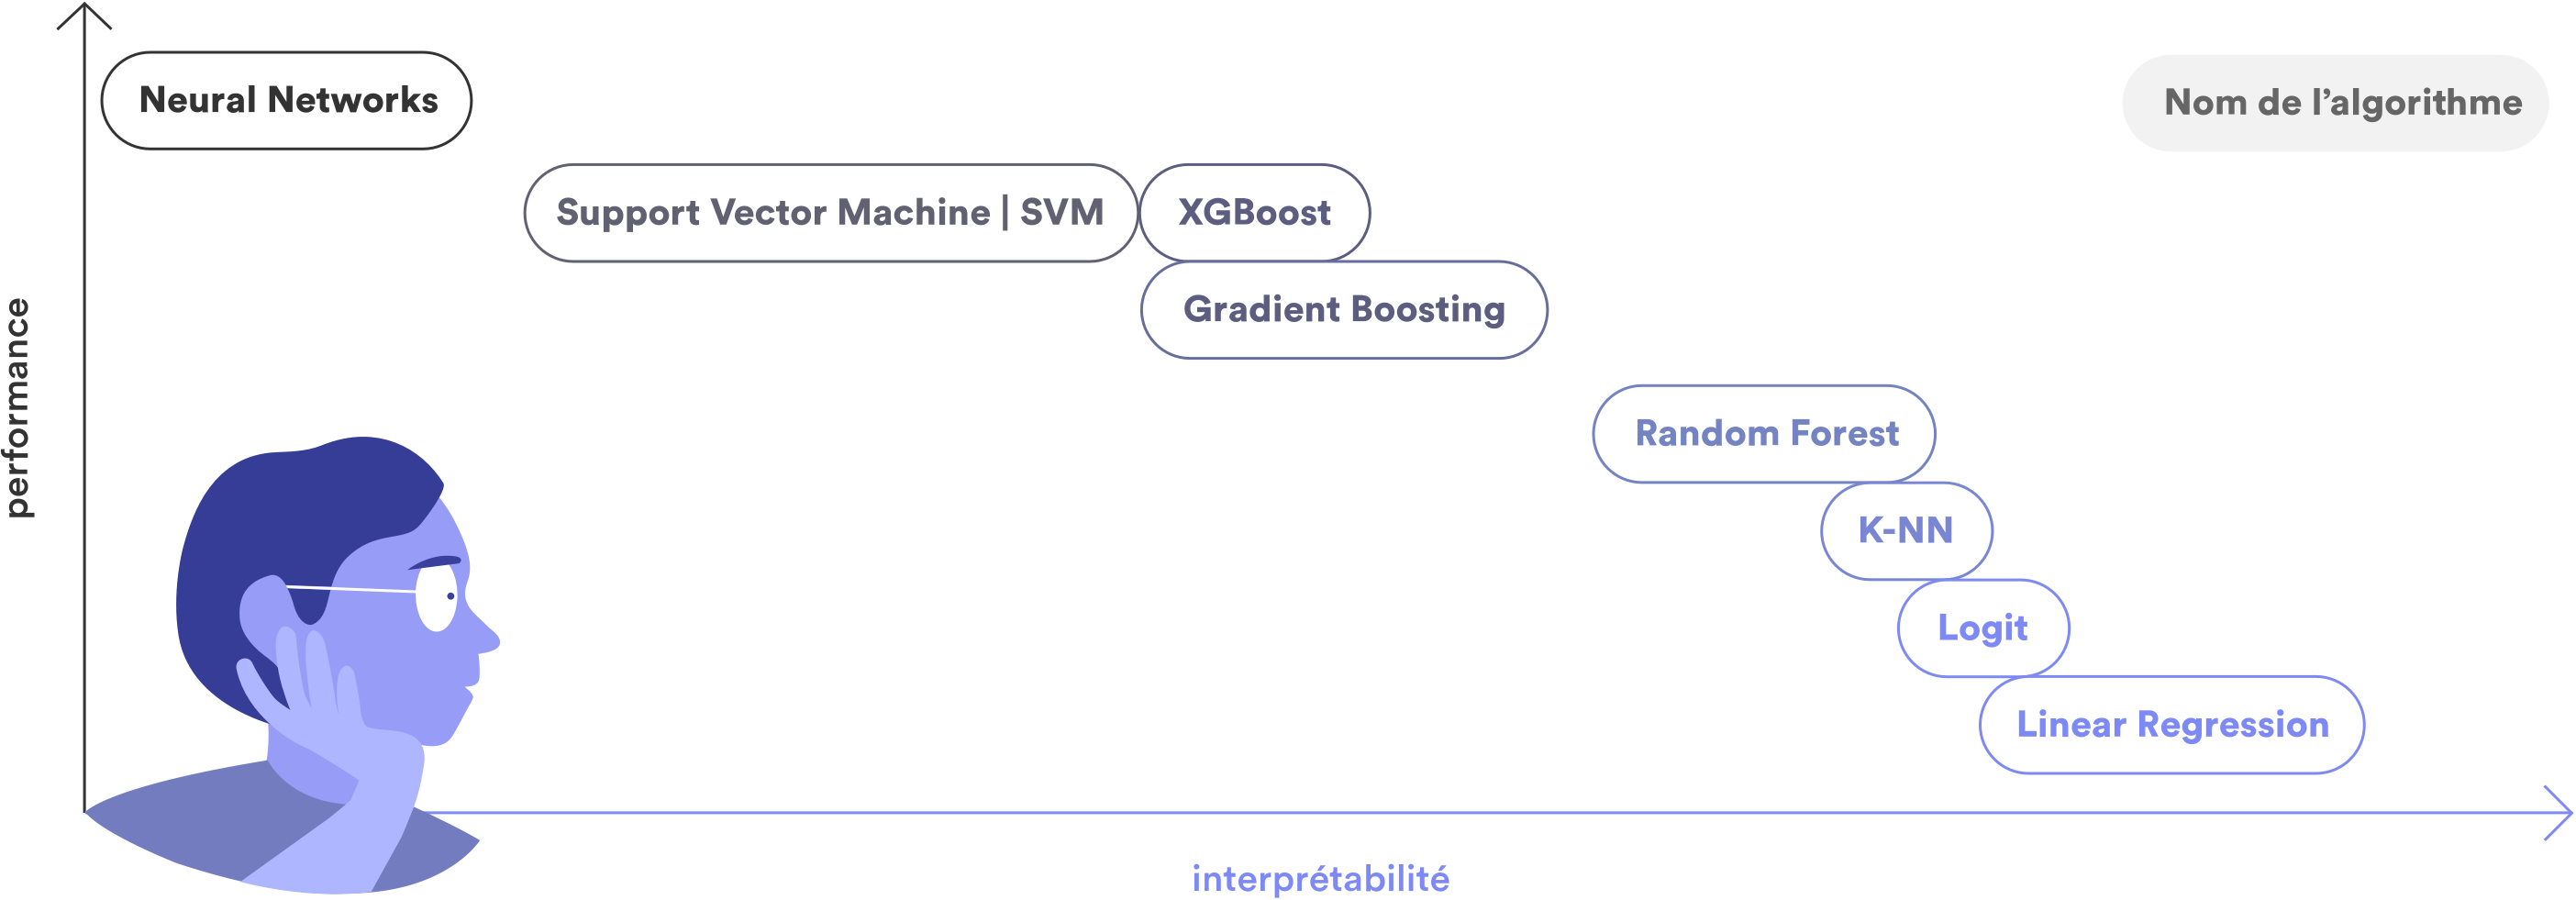
\includegraphics[scale=0.15]{src_img/performanceAndInterpretabilite.png}
\caption{Lien entre la performance et l'interprétabilité d'un algorithme de machine learning. \textit{Source : https://hippocrate.tech/}}
\label{performanceAndInterpretabilite}
\end{figure}

À l'heure actuelle, le réseau de neurones artificiel fait partie des algorithmes les plus performante et aussi est le plus couramment utilisée.
La non-explicabilité de ces modèles posent des problèmes de fiabilité, d'éthique et de responsabilité. Ce floue accentue aussi la méfiance et la peur des personnes envers l'intelligence artificielle, et entraîne un problème de compréhension entre les Data Scientist et les expert métier qui en plus de ne pas comprendre comment fonctionne le modèle ne comprennent pas non plus son résultat. Aussi, expliquer ces modèles permettrai d'améliorer notre conformité à la loi ainsi que d'augmenter les performances de nos modèles. Cette nouvelle problématique présente donc de nombreux enjeux de tailles.\par

\subsection{L'éthique}
Tout d'abord, de nombreux cas très exposés dans les médias nous montrent que cette incompréhension peut amener à des problèmes du point de vue éthique. La question de l'éthique est souvent ramenée à deux aspects principaux : la discrimination et la protection des données privées des usagers.
\subsubsection{La discrimination}
La question essentielle à se poser est de savoir comment une intelligence artificielle est amenée à prendre des décisions discriminante. Dans un article, Barocas et Selbst distinguent cinq façons par lesquelles une intelligence artificielle pourrait aboutir à une discrimination \cite{discriminationWay}. Ces cas sont uniquement des cas involontaires et ne prennent pas en compte une discrimination délibérée qui pourrait bien évidemment être possible.
\begin{itemize}
    \item \textbf{Définition des variables cibles et des étiquettes de classes} : le but d'une intelligence artificielle est de découvrir des corrélations dans des jeux de données. Ainsi, certain choix de variables cibles ou ou d'étiquettes de classes peuvent amener à faire des corrélations discriminatoire. Un exemple trivial serait de considérer un modèle permettant de savoir si un employé fait du travail de qualité, l'entreprise choisira de prendre en compte les retards des employés dans son modèle d'évaluation. Les personnes défavorisées habitant souvent loin de leur lieu de travail, ont plus souvent tendance à être en retard à cause des embouteillages et des problèmes de transport. Ces employés habitant loin, seront jugés comme faisant du travail de moins bonne qualité ce qui n'est pas forcément le cas. Si on ajoute à cela le fait que les personnes issus de l'immigration sont en moyenne plus pauvre et habitent en moyenne plus loin des centres villes, nous pouvons arriver involontairement à une IA discriminante par le simple fait d'utiliser l'étiquette "retard" dans l'évaluation des performances d'un employé.
    \item \textbf{Les données d'apprentissage} : les données d'apprentissage peuvent contenir des biais qui seront ensuite appris par notre modèle. L'exemple de l'IA de recrutement de l'entreprise Amazon qui rejetait les CVs contenant le mot "femme" évoqué en introduction le montre bien. Cette IA avait appris en analysant tous les profils recrutés par Amzon dans le passé, or les personnes recrutées étaient très majoritairement des hommes. L'IA a donc déduis qu'il était préférable de recruter des hommes. 
    \item \textbf{La collecte des données d'apprentissages} : Les lieux dans lesquels sont récoltées les données d'apprentissage sont aussi déterminant. Par exemple si l'on récolte des données concernant la criminalité dans un quartier avec des personnes issus majoritairement de l'immigration, l'IA aura plus tendance à considérer les immigrés comme de potentiels criminels par rapport aux personnes non-imigrées et inversement si on choisis un quartier avec des personnes majoritairement non-imigrées.
    \item \textbf{La sélection des caractéristiques} : Afin que l'IA puisse s'entraîner, il faut lui fournir des données qui sont en réalité une représentation simplifiée de notre monde. Ainsi, son créateur doit faire des choix pour sélectionner les caractéristiques qui constitueront cette représentation. Ce choix peut par concours de circonstance involontairement découler sur de la discrimination il faut donc les choisir avec parcimonie.
    \item \textbf{Données indirect} : Certaines données peuvent inclure des données indirect. Par exemple : \textit{"un jeu de données qui ne contient pas de données explicites sur l’orientation sexuelle peut tout de même la dévoiler. Une étude de 2009 a montré que les liens d’"amis" sur Facebook révèlent l’orientation sexuelle par une méthode de prédiction précise de l’orientation sexuelle des utilisateurs de Facebook fondée sur l’analyse de leurs liens. Le pourcentage d’"amis" s’identifiant comme homosexuels serait fortement corrélé avec l’orientation sexuelle de l’utilisateur concerné"}\footnote{Frederik Zuiderveen Borgesius, Discrimination, intelligence artificielle et décisions algorithmiques}. 
\end{itemize}
Mieux comprendre le fonctionnement de nos algorithmes permettrait donc de mieux se prémunir des discriminations involontaires. Aussi on pourrait prendre en compte l'explication en plus de la prédiction afin de fournir un résultat optimal. Par exemple, aux États-Unis, un algorithme appelé Compas est utilisé par les juges pour évaluer la probabilité pour un prévenu de se faire arrêter à nouveau dans les deux ans à venir. Cet algorithme est beaucoup remis en cause, car il est jugé "non-pertinant" et "discriminatoire" par certaines personnes alors que d'autres ont grandement confiance en lui, deux camps s'affrontent donc. Dans ce cas-là, fournir une explication conjointement à la prédiction permettrai de mettre tout le monde d'accord, ainsi nous pouvons prendre en compte la prévision et déterminer si dans le cas précis elle est issue d'un jugement non-pertinant, discriminatoire ou autre.
\subsubsection{Protection des données}
L'apprentissage d'une intelligence artificielle requière un très grand nombre de données, parmi lesquelles peuvent se trouver des données personnelles. L'utilisation d'un modèle pourrait donc aussi nécessiter de fournir des données personnelles afin d'effectuer une prédiction. L'utilisation de ces données jugées critiques est problématique, car des restrictions et des règles de protection en découlent. Tel qu'évoqué dans l'introduction, le RGPD par l'addition de plusieurs de ses articles implique un "droit à l'explication". Ce droit a été démontré par Seth Flaxman et Bryce Goodman \cite{RGPDexplanRight}, ce qui a donc pour effet d'accentuer le besoin d'applicabilité des modèles de décision boites noires. En effet, pour le moment ce droit est inaccessible par les usagers et les entreprises éprouvent des problèmes de responsabilités.

\subsection{Fiabilité et confiance}
Deuxièmement, expliquer les décisions prisent par un modèle boite noire permettrai d'augmenter la fiabilité que l'on lui accorde. Le modèle peut très bien fonctionner dans la plupart des cas, mais il est possible qu'il réagisse mal dans un certain cas bien spécifique. Avec l'absence de compréhension du fonctionnement interne de notre modèle, nous pouvons ne pas prévoir ce cas spécifique qui représente un risque. Le domaine médical par exemple est en attente d'une plus grande fiabilité de ses modèles en effet, une erreur peut avoir des conséquences graves et mettre en danger des personnes. La manière classique de mesurer la fiabilité d'un modèle est de calculer sa précision (accuracy), cela consiste à diviser le nombre de prédictions corrects par le nombre de prédiction total. Cette méthode indispensable ne permet pas à elle seule une fiabilité optimal en notre modèle, admettons que nous arrivons à une précision de 100\% rien ne nous dis que dans un cas très particulier notre modèle ne nous donnera pas une prédiction fausse. La compréhension de la logique interne de notre modèle serai donc un facteur supplémentaire dans la fiabilité que l'on lui donne. \par
De plus, un soudage publié par OpinionWay\footnote{https://www.opinion-way.com/fr/} montre que 30\% des Français ont peur d'un jugement porté par l'intelligence artificielle dans le domaine financier et 21\% dans le domaine médical. L'incompréhension de la logique interne des algorithmes décisionnels tend à accentuer la méfiance envers ces technologies. Fournir une explication permettrai d'augmenter l'acceptation de ces nouvelles technologies.

\subsection{Performance}
Enfin, expliquer la logique interne de la boite noire permettrai d'améliorer le développement de celle-ci, de la rendre plus compétitive et plus performante. Ces explications seront aussi utiles durant leur développement afin de comprendre pourquoi notre modèle ne fonctionne pas bien dans certains cas voir même pourquoi il ne converge pas du tout.

\section{Interprétabilité et explicabilité}

Dans le domaine du machine learning, les mots interprétabilité et explicabilité sont très souvent utilisés conjointement et il peut être difficile au premier abords d'en saisir la différence. De plus, il existe de nombreuses définitions différentes pour ces termes et tous les experts ne s'accordent pas forcement à ce sujet. Après l'analyse de différentes propositions, nous nous accorderons, dans ce mémoire, à donner les définitions suivantes :\par
L'interprétabilité est le fait de pouvoir observer l'effet d'une cause dans un système c'est-à-dire de pouvoir prédire les changements dans la sortie lorsque l'on change une variable d'entrée.\par
L'explicabilité, quant à elle, est le fait d'expliquer dans des termes compréhensibles par l'homme la mécanique interne de notre système.\par
Afin de bien saisir la différence, le site \textit{KDnuggets} dans un article du nom de "Machine Learning Explainability vs Interpretability: Two concepts that could help restore trust in AI"\footnote{https://www.kdnuggets.com/2018/12/machine-learning-explainability-interpretability-ai.html} nous invite à voir les choses comme si nous faisons une expérience scientifique à l'école : L'expérience peut être interprétable dans la mesure où vous pouvez voir ce que vous faites, mais elle n'est vraiment explicable qu'une fois que vous avez creusé la chimie derrière ce que vous pouvez voir se produire.\par
Créer un modèle interprétable implique de prendre en compte plusieurs facteurs :\par
\begin{description}
\item[Interprétabilité globale et local] L'interprétabilité d'un modèle est dite \textit{globale}, lorsque l'on comprend sa logique dans la totalité, nous sommes donc en mesure d'en expliquer toutes les solutions. À contrario, elle sera dite \textit{local}, lorsqu'il est possible d'expliquer seulement une ou plusieurs solutions spécifiques. Un problème complexe pourra ainsi être découpé en un sous problème plus simple afin de pouvoir expliquer une partie des solutions comme le montre la figure 1.2 ci-dessous.
\begin{figure}[h]
\centering
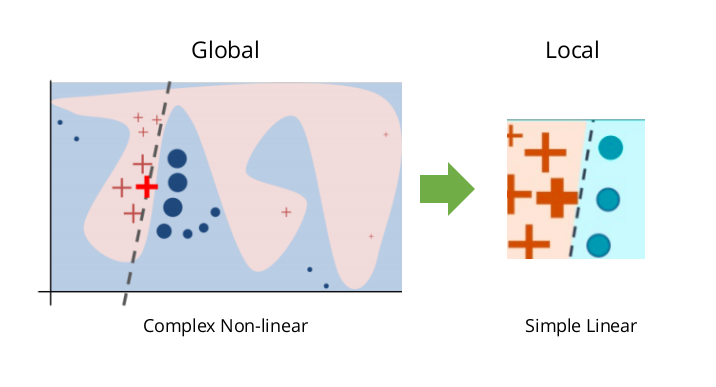
\includegraphics[scale=0.4]{src_img/globalVSlocal.png}
\caption{Un problème global complexe pouvant être expliqué à échelle local. \textit{Source : www.kdnuggets.com}}
\label{globalVSlocal}
\end{figure}

\item[Limatation temporel] Le temps que l'on peut allouer pour fournir une explication à notre modèle est aussi à prendre en compte. En effets, fournir une explication peut prendre du temps et cette explication peut être longue à appréhender pour un être humain. Dans certains contextes où la prise de décision devra être effectuée rapidement, il sera préférable d'avoir une explication simple, compréhensible et fournis rapidement par la machine. Dans d'autres cas, nous pourrons prendre le temps d'aborder une explication plus complexe et détaillée.

\item[La cible de l'explication] La nature de l'expertise de l'utilisateur est aussi un facteur à prendre en compte dans le choix de l'explication que nous voulons lui apporter. En effets, un expert dans le domaine aura tendance à préférer une explication exhaustive et précises qu'une explication simple et opaque et inversement pour une personne moins à l'aise.
\end{description}

\subsection{Pré-requis d'un modèle interprétable}
En plus de prendre en compte les facteurs précédemment évoqués, un modèle interprétable doit être capable de satisfaire une liste de choses souhaitées. L'article "A survey of methods for explaining black box models"\cite{surveyExplaining} met en avant, après une analyse de différents états de l'art traitant de ce sujet, les desiderata d'un modèle interpretable :
\begin{description}
\item[Interpretabilité] Dans quelle mesure le modèle ou la prédiction sont compréhensifs par l'homme. Ce sujet est encore en débat afin de savoir comment mesurer cette interprétabilité.

\item[Précision] Dans quelle mesure le modèle interprétable prédit avec précision les différentes instances. La précision d'un modèle peut être faite avec le \textit{score de précision} (accuracy score), il s'agit simplement d'un rapport entre les observations correctement prédites et les observations totales. La précision est l'indicateur de base afin de calculer la précision d'un modèle, ce score fonctionne mieux si les faux positifs et les faux négatifs ont un coût similaire. Si le coût des faux positifs et des faux négatifs est très différent, il vaut mieux regarder le \textit{F1-score}. Le F1-score est la moyenne pondérée de la précision et du rappel.
\[
F1 Score = 2*\frac{Recall * Precision}{Recall + Precision}
\]
Où la \textit{précision} est le rapport des observations positives correctement prédites au total des observations positives prévues. Et le \textit{recall} (rappel) est le rapport des observations positives correctement prédites à toutes les observations dans la classe réelle.

\item[Éthique] Si notre modèle traite des données personnelles, il devra garantir en plus une protection contre toutes formes de discrimination ainsi qu'une protection de la vie privée des personnes concernées.\\
\end{description}

Ces différents aspects jouent un rôle important quant à la confiance qu'un utilisateur va apporter à notre modèle interprétable. De plus d'autres notions viennent s'ajouter, notamment pour les modèles d'exploration de données et d'apprentissage automatique. Il est important de respecter des critères tels que la \textit{robustesse}, la \textit{causalité}, l'\textit{évolutivité} et la \textit{généralité}. Cela signifie qu'un modèle doit garantir un certain niveau de performance indépendamment des données d'entrée (robustesse), et que les changements d'entrée dû à une perturbation affectent le comportement du modèle (causalité). Enfin, étant donné que nous pouvons utiliser le même modèle avec une multitude données d'entrée et dans différents cas d'applications, il est préférable d'avoir des modèles portables possédant un minimum de restriction (évolutivité, généralité).

\section{Ouvrir les boites noires}
L'article "A survey of methods for explaining black box models"\cite{surveyExplaining} passe en revue cinquante-quatre méthodes aillant pour but d'ouvrir différentes boites noires, en nous fournissant une classification exposée dans un tableau disponible en annexe 1 et 2. Nous aurons l'occasion de reparler de ce tableau plus tard. Cette revue permet de distinguer différents types de problèmes, d'explicateurs, de boites noires, de données d'entrée ainsi que différentes restrictions sur le modèle (accès au code, aux données...). Nous allons commencer par expliquer ces différentes caractéristiques.

\subsection{Types de problèmes}
\subsubsection{Explication du modèle}
Ce problème consiste à fournir un modèle interprétable et transparent capable d'imiter le comportement d'une boite noire et de nous fournir un prédicat compréhensible par l'homme.\\
Étant donnée un prédicateur de boite noire b et un ensemble de données D, le problème d'explication du modèle consiste à trouver une fonction f telle que f(b,D)=c où c est un prédicateur compréhensible capable d'imiter le comportement de b et dérivable afin d'obtenir une explication.

\subsubsection{Explication du résultats}
Ce problème consiste à fournir un résultat interprétable, c'est-à-dire que le modèle devra fournir le résultat avec une explication sur les raisons qui l'ont poussé à donner cette prédiction. Il n'est pas nécessaire d'expliquer la logique interne du système mais seulement le processus de décision pour une instance donnée (interprétation local).

\subsubsection{Inspection de la boîte noire}
Ce problème consiste à fournir une représentation visuelle ou textuelle afin de comprendre le fonctionnement interne de notre boite noire.\\
Étant donnée un prédicateur de boite noire b et un ensemble de données D, le problème d'explication du modèle consiste à trouver une fonction f telle que f(b,D)=V où V est une représentation du fonctionnement de la boite noire.

\subsubsection{Conception transparente}
Ce problème consiste à fournir un modèle transparent qui soit directement interprétable globalement ou localement.

\subsection{Types d'explicateurs}
\begin{itemize}
    \item \textbf{Arbre de décision (Decision Tree)} : L'arbre de décision exploite un arbre qui a pour noeuds des conditions, les arrêtes correspondent à la valeur d'une variable d'entrée et les feuilles correspondent aux différents labels possible. La figure 1.3 montre un exemple trivial d'arbre de décision. Ainsi, la décision sera simplement expliquée en exprimant les chemins de l'arbre empruntés. 

    \begin{figure}[h]
    \centering
    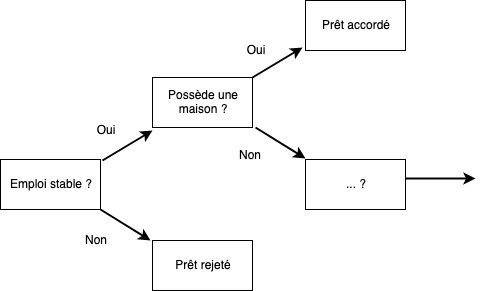
\includegraphics[scale=0.5]{src_img/decision_tree.jpg}
    \caption{Exemple d'un arbre de décision}
    \label{decision_tree}
    \end{figure}
    
    \item \textbf{Règles de décision (Decion Rules)} : Utilisé pour expliquer le modèle, le résultat ainsi que pour la conception transparente. Il est aussi possible de transformer un arbre en un ensemble de règles. Les règles de décisions sont simplement des conditions IF-THEN : 
    
    if condition1, condition2, condition3 then outcome 
    
    \item \textbf{Importance des fonctionnalités (Features Importance)} : Solution souvent utilisée, elle consiste à trouver les entrées de la boite noire pour lesquelles les poids sont les plus importants. Par exemple, pour une classification d'image, de trouver les pixels les plus importants dans l'entrée pour en arriver à une prédiction. Comme le montre la figure 1.4 tirée de l'article \textit{"Explainable Artificial Intelligence: Understanding, Visualizing and Interpreting Deep Learning Models"} \cite{explainingIA}.\\
    \begin{figure}[h]
        \centering
        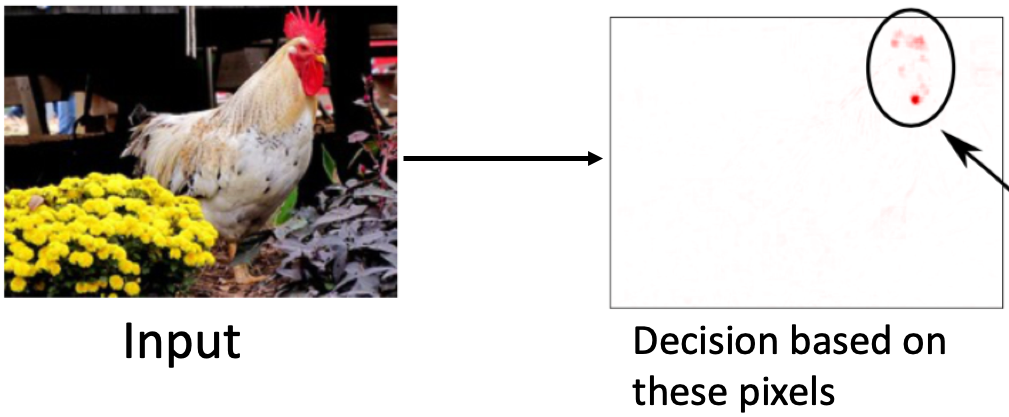
\includegraphics[scale=0.35]{src_img/chickenPixel.png}
        \caption{Importance des fonctionnalités : explication de la prédiction "coq"}
        \label{chickenPixel}
    \end{figure}
    
    \item \textbf{Salient Mask} Généralement utilisé pour expliquer localement les réseaux de neurones profond (DNN), le salient mask permet de mettre en évidence visuellement les parties déterminantes de l'entrée analysée. L'article \textit{"Real Time Image Saliency for Black Box Classifiers"}\cite{silentMask} décrit son fonctionnement et la figure 1.5 montrant un exemple de salient mask est tirée de cet article.
    \begin{figure}[h]
        \centering
        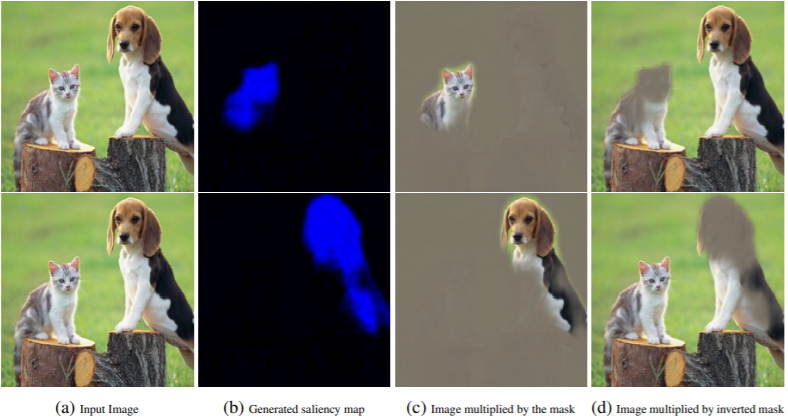
\includegraphics[scale=0.85]{src_img/silentMaskExemple.PNG}
        \caption{Masque saillant : explication de la prédiction chien et chat}
        \label{silentMaskExemple}
    \end{figure}
    
    \item \textbf{Analyse de sensibilité (Sensitivity Analysis)} : Généralement utilisée pour l'inspection de boite noire. L'analyse de sensibilité consiste à évaluer l’incertitude statistique du résultat d’une boîte noire avec les différentes sources d’incertitude dans ses entrés. En d'autres termes, cela consiste à modifier des variables d'entrées afin de voir si cela a un impact sur le résultat en sorti et donc de savoir comment elles affectent notre prédiction.
    
    \item \textbf{Diagramme de dépendance partielle (Partial Dependence Plot)} : Ces graphiques permettent de comprendre l'effet d'une ou deux variables d'entrée sur la sortie du modèle. Le but étant de  montrer si la relation entre une caractéristique d'entrée et la sortie est linéaire, monotone ou plus complexe. Par exemple, appliqué à un modèle de régression linéaire, les tracés de dépendance partielle montrent toujours une relation linéaire. Nous somme limité par une ou deux variables à la fois, car une variable donne une représentation en 2 dimensions du problème et deux variables fournissent donc une représentation 3 en dimensions. Par exemple, la figure 1.6 tirée du livre \cite{molnar2019} montre trois diagrammes de dépendances différents sur trois valeurs d'entrées (la température, l'humidité et la vitesse du vent) et leurs impactes linéaire sur la prédiction du nombre de vélos.
    \begin{figure}[h]
        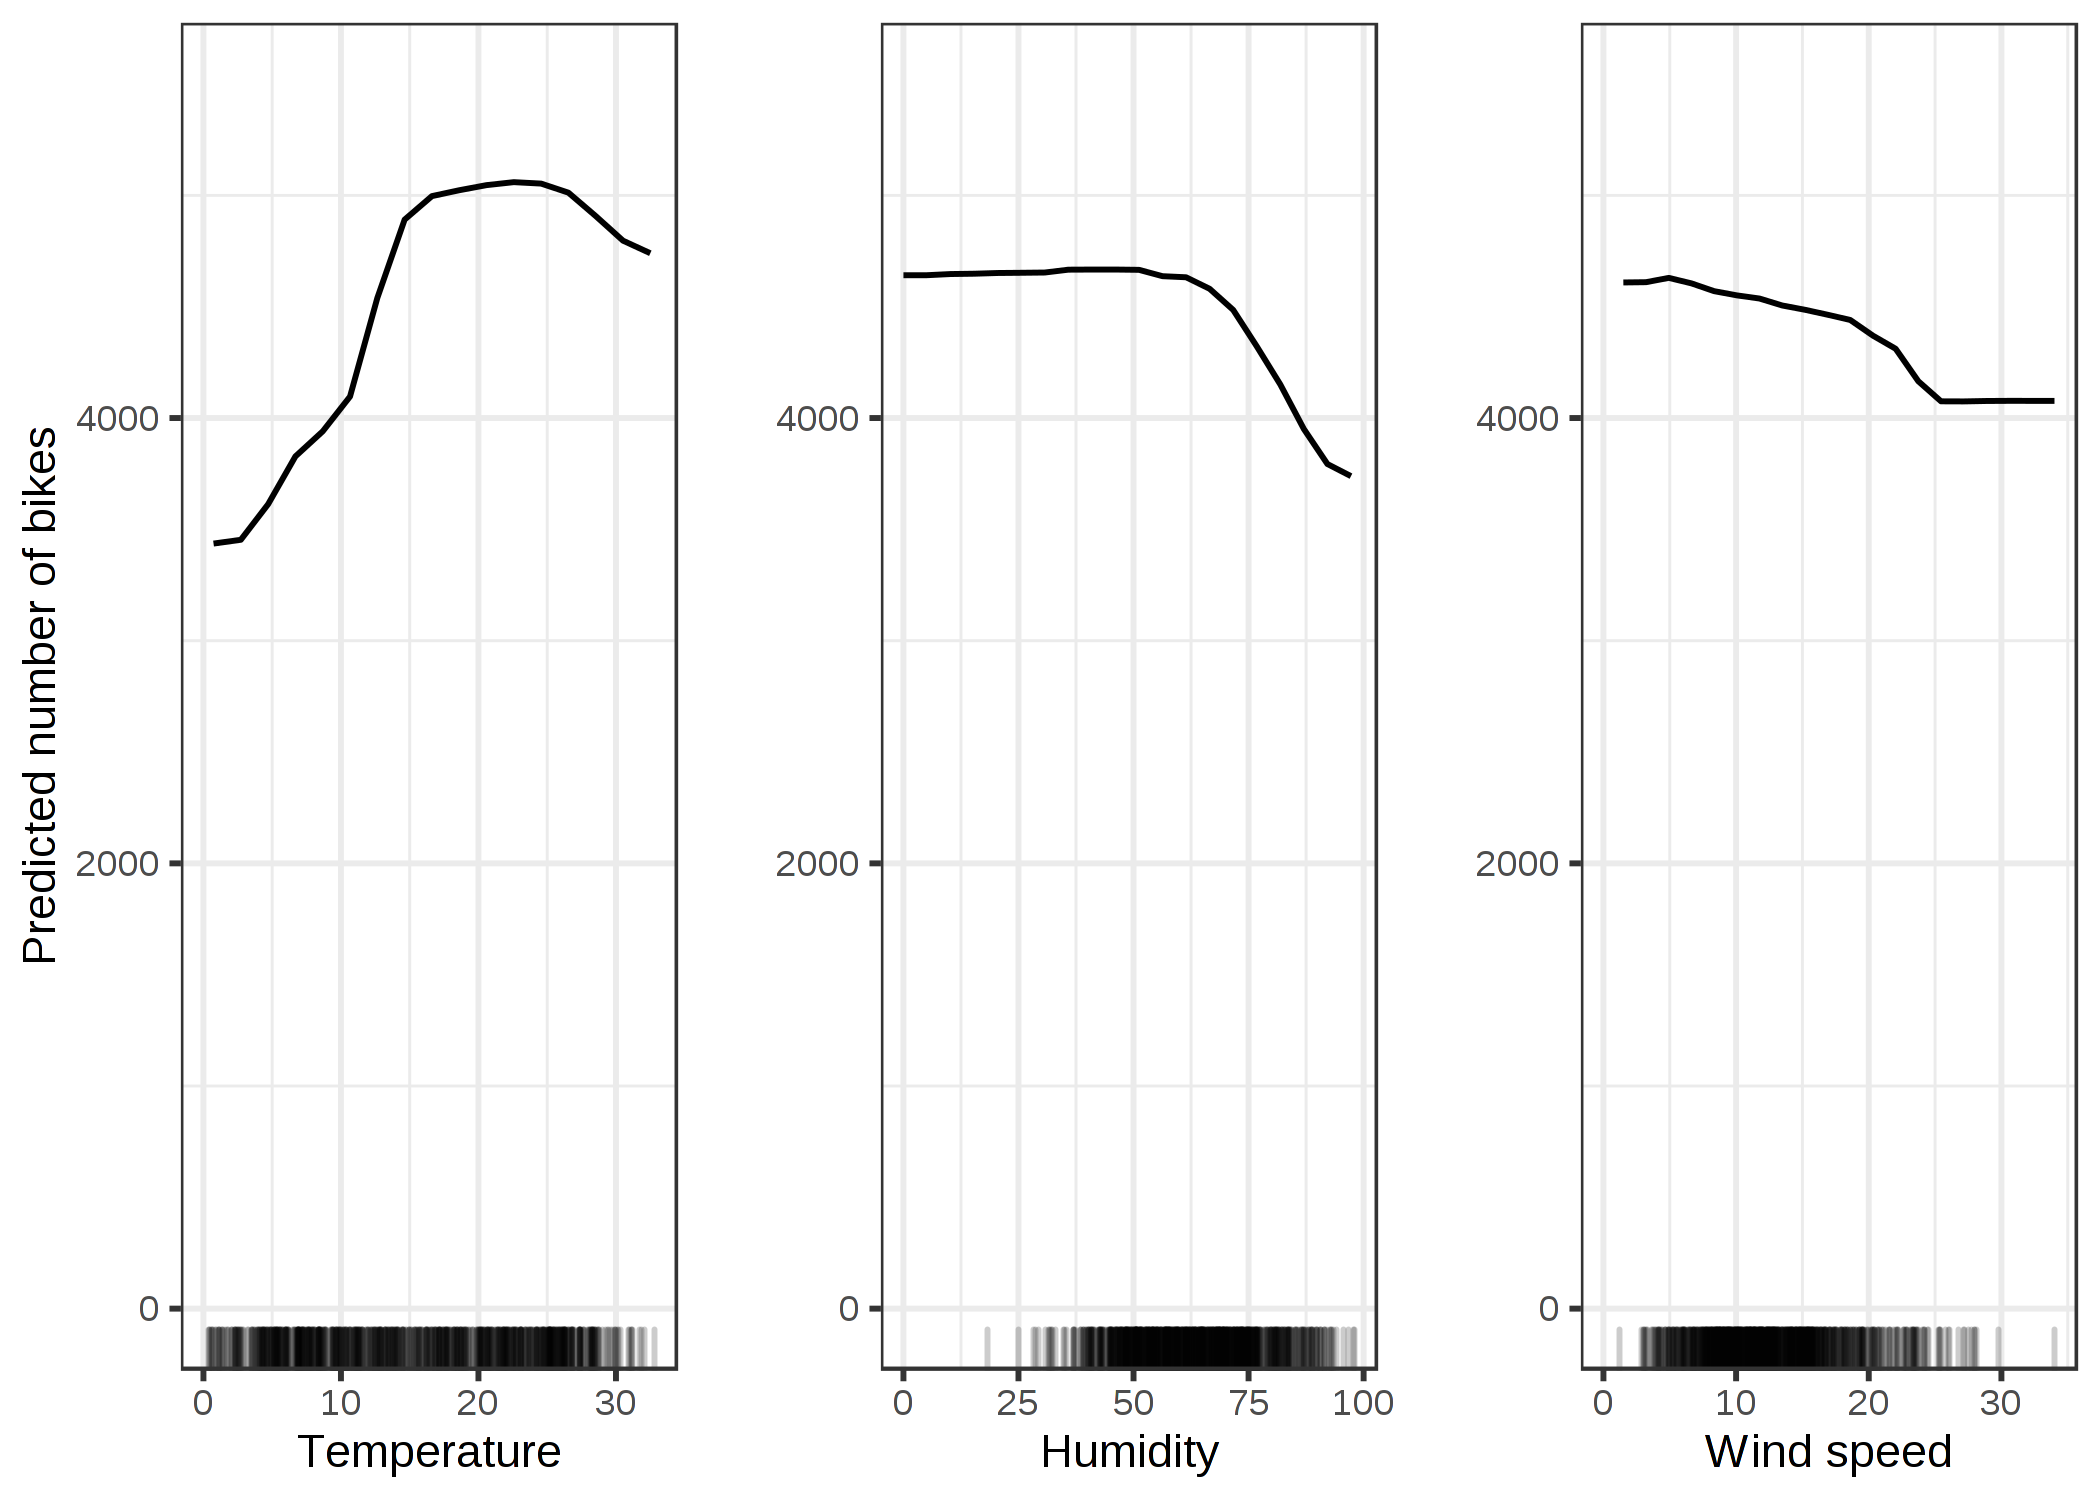
\includegraphics[scale=0.17]{src_img/partialDependencePlot.png}
        \caption{Exemple de diagramme de dépendance partielle.}
        \label{partialDependencePlot}
    \end{figure}
    
    \item \textbf{Sélection de prototype (Prototype Selection)} : Cet explicateur consiste à retourner, avec le résultat, un exemple très similaire à l'enregistrement classifié, afin de préciser avec quel critère la prédiction a été renvoyée.
    
    \item \textbf{Activation des neurones (Neurons Activation)} : L'analyse des réseaux de neurones permet aussi de comprendre son comportement. Cela consiste à analyser les neurones activés pour chaque entrés passées en argument à notre modèle.
\end{itemize}

L'explicateur varies en fonction de notre type de problème, de notre type de boite noire, de notre type de données d'entrée (images, texte...) et de nos différentes restrictions sur le modèle (accès au code, aux données...).

\section{Approches utilisées}
Face à ce besoin d'explicabilité grandissant, les entreprises peuvent préférer se tourner vers des modèles moins performant mais plus explicable afin de contourner la problématique de boite noire. Ainsi, nombreuse sont les entreprises qui se détournent de l'apprentissage profond au profil de l'apprentissage par arbre de décision ou les modèles linéaires par exemple qui fournissent un résultat plus compréhensibles et interprétable. Mais, la recherche dans ces domaines n'a pas évoluée depuis un certain temps et l'éventail des algorithmes disponibles est assez limité.

\subsubsection{Sur-couche explicative}
Le but étant d'essayer de fournir à l'utilisateur des éléments approximatifs permettant de comprendre son modèle boite noire, comme par exemple identifier les variables d'entrée les plus importantes dans la prise de décision du modèle. Comme le montre la figure 1.7, la sur-couche explicative vient se greffer après la prédiction du modèle.
\begin{figure}[h]
\centering
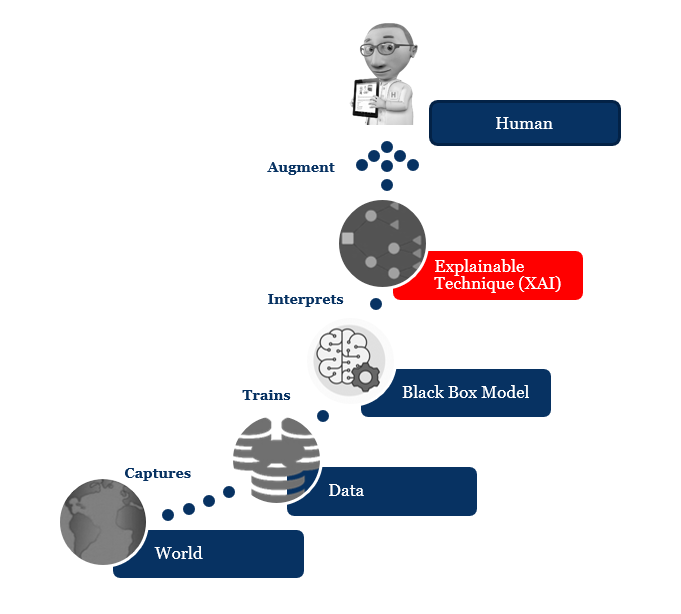
\includegraphics[scale=0.35]{src_img/explainCouche.png}
\caption{Position de la sur-couche explicative dans le processus de prédiction. \textit{Source : www.kdnuggets.com}}
\label{explainCouche}
\end{figure}
Différents outils proposent une approche permettant de livrer des éléments de compréhension approximatif pour un modèle boite noire simple. Nous allons présenter les deux outils les plus populaires, LIME et SHAP.
\subsection{LIME}
LIME signifie Local Interpretable Model-Agnostic Explanations (explications locales interprétables par modèle-agnostique). L'objectif est donc de fournir une interprétation local à un modèle de classification ou de régression (model agnostic) en se basant sur l’importance des variables comme vu précédemment. L'idée est de sonder la boite noire autant de fois que nécessaire en faisant varier les données d'entrées ce qui aura pour effet de produire une nouvelle sortie à chaque fois. Une fois toutes les perturbations sont effectuées il est alors possible de récupérer les coefficients qui composent la droite de la régression linéaire et ainsi de déduire l'importance des variables d'entrées. Par exemple dans la figure 1.8 tirée de l'article original de la présentation de LIME\cite{limePaper} : L'image originelle (a) est donnée à notre boite noire qui prédit "Guitare électrique", "Guitare acoustique" et "Labrador". Nous constatons que le modèle s'est trompé sur la reconnaissance de la guitare électrique et nous utilisons LIME afin de comprendre ce qu'il s'est passé. LIME va prendre notre image (a) et la dériver de plusieurs façons en cachant certaines parties et envoyer ces nouvelles images à notre modèle. Le but étant de trouver les parties qui une fois cachées font que le modèle ne prédit plus la même chose. Puis une fois les trois classes trouvées, LIME nous envoie une explication où l'on voit les parties de l'image aillant joué un rôle dans la prédiction de chaque labels de notre modèle.
\begin{figure}[h]
\centering
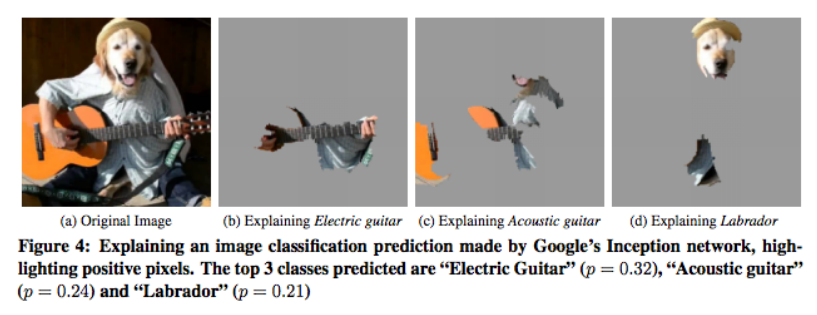
\includegraphics[scale=0.35]{src_img/limeExemple.png}
\caption{Source : LIME Paper}
\label{limeExemple}
\end{figure}

\subsection{SHAP}
Un an après la sortie de LIME, un nouvel outil fait son apparition afin de compenser ses quelques défauts, cet outil s'appelle SHAP. SHAP signifie SHapley Additive exPlanations, c'est une méthode permettant de fournir une interprétation local à une prédiction. Cette méthode est basée sur la valeur de Shapley issus de la théorie des jeux, il est donc nécessaire dans un premier temps d'expliquer brièvement cette valeur de Shapley.\par
La valeur de Shapley introduit par Shapley en 1953, permet de repartir les gains équitablement dans un jeu coopératif. Le but étant que tous les joueurs coopérant ensemble reçoivent un certain gain en fonction de leur contribution.\par
SHAP reprends cette idée afin d'expliquer toutes sortes de modèle de machine learning, le but étant d'associer une valeur égale à sa contribution dans la prédiction pour chaque caractéristique d'entrée. Prenons par exemple un modèle permettant de prédire le prix d'un logement. Une multitude de caractéristiques sont données en entrés à notre modèle afin d'estimer le prix du logement, le but de SHAP est donc de définir pour chacune de ces caractéristiques leur impact monétaire sur le prix final du logement. Il interrogera donc la boite noire avec une multitude de cas différents afin d'isoler le prix de chaque caractéristique. Prenons le cas de la figure 1.9 où l'on veut expliquer la prévision de 310 000 euros pour un logement de 50m2, au premier étage, près d'un parc et où les animaux sont interdits. SHAP va donc recréer la même l'instance et la donner en entrée à la boite noire en autorisant les animaux afin d'en déduire le coût (dans notre exemple 10 000 euros). Cette opération sera effectuée sur toutes les caractéristiques du problème afin de trouver la contribution de chacune. Cela peut sembler trivial dans cet exemple mais il peut exister des dépendances entre les caractéristiques qui modifient leurs coût en fonction de la présence ou non d'une ou plusieurs autre(s) caractéristique(s).
\begin{figure}[h]
\centering
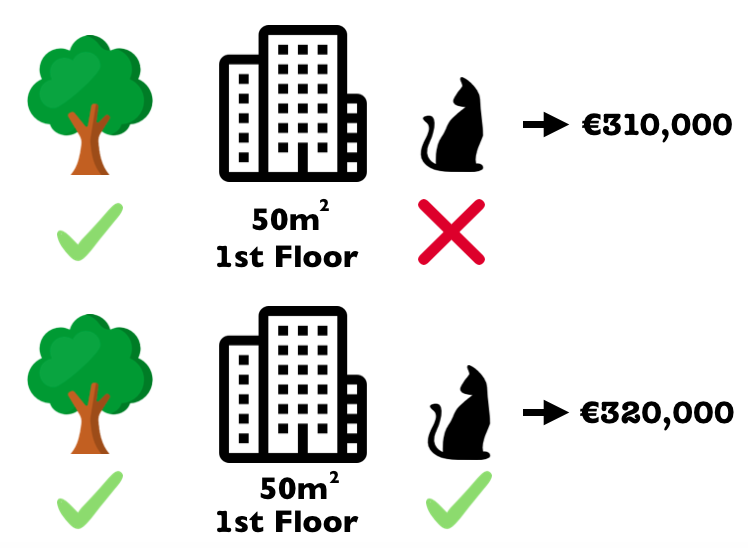
\includegraphics[scale=0.3]{src_img/shapleyExemple.png}
\caption{Exemple de l'explication du coût d'un logement avec SHAP. \textit{Source : Christoph Molnar, Interpretable Machine Learning}}
\label{shapleyExemple}
\end{figure}

\subsection{Limites de ces implémentations}
Aujourd'hui, de nombreuses implémentations de ces méthodes sont utilisées, mais elles essuient aussi quelques critiques et ne conviennent pas dans tous les cas de figures. Premièrement, ces algorithmes représentent un coût non négligeable. Ces méthodes basées sur des simulations et interrogeant notre modèle plusieurs fois pour une seule prédiction, peuvent poser des problèmes de performances lorsque l'on manipule un très grand nombre de données. Aussi la pertinence des explications fournies sont sujettes à débat, en effet ce sont des approximations et rien ne nous garantis que ces explications correspondent réellement au fonctionnement de notre modèle. Ces explications pourraient même donner l'effet inverse à celui escompté, en effet on peut arriver dans des cas où l'on fait confiance à notre modèle grâce à ces explications alors qu'elles ne sont pas fondées et ainsi prendre une décision critique appuyée sur une explication erroné.\par

Il est donc nécessaire d'utiliser ces algorithmes avec parcimonie et en aillant bien conscience qu'ils ne fournissent que des approximations de notre problème. Mais ce genre d'approches sont très bénéfiques pour la recherche, elles nous permettent d'apporter de nouvelles solutions ainsi que de mettre en lumière de nouvelles problématiques.


\chapter{Application}
Nous avons vu dans le chapitre 1 de ce mémoire que l'utilisation d'algorithmes de type boites noires dans l'aide à la prise de décision soulevait des questions, notamment sur l'éthique, la fiabilité et la performance. Dans cette partie, nous allons mettre en application nos recherches présentées dans l'état de l'art afin de déterminer si l'interprétabilité d'un modèle boîte noire nous permettrai de résoudre ces problèmes.
\section{Mise en évidence de biais}
L'objectif de cette partie est de démontrer que rendre un modèle boite noire interprétable permettrai de mettre en évidence des biais discriminatoire. Pour cela, nous allons créer un modèle prédictif à partir d'un jeu de données comportant possiblement des biais, puis d'utiliser l'outil SHAP afin d'essayer de mettre en évidence les éventuels biais présents dans notre jeu de données. Le code de cette section est disponible sur mon GitHub \cite{shapMyDepot} et suit, entre autre, le tutoriel de "Towards Data Science"\cite{shapTuto}
\subsection{Le jeu de données}
Afin de savoir si utiliser une méthode de compréhension de boites noires aurai permis de mettre en évidence les biais présents dans l'intelligence artificielle dite sexiste de l'entreprise Amazon (évoquée dans l'introduction de ce mémoire), nous appliquerons ces méthodes sur un exemple similaire. Pour rappel, cette IA rejetait les CVs de femmes car elle avait été entraînée en se basant sur les personnes employées par l'entreprise dans le passé et que ces personnes étaient majoritairement des hommes, l'IA a donc conclue qu'il était préférable d'embaucher un homme plutôt qu'une femme.\par
Pour cette expérimentation, nous allons utiliser un jeu de données qui nous donne des informations sur des étudiants ainsi que leurs notes à différents examens. Les données d'entrée de notre modèle seront donc de type tabulaire. Ce jeu de données disponible ici \cite{examScore} ressemble à cela (Figure \ref{studentsPerformanceDataSet}) :

\begin{figure}[h]
    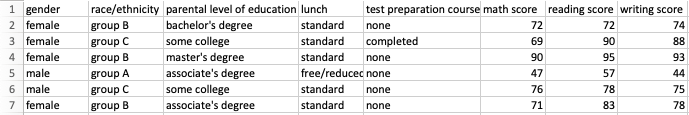
\includegraphics[scale=0.65]{src_img/studentsPerformanceDataSet.png}
    \caption{Jeu de donnée des performances des étudiants}
    \label{studentsPerformanceDataSet}
\end{figure}

À noter, que ce jeu de données est fictif et généré aléatoirement. Notre but est de créer un modèle qui prédira la moyenne d’un étudiant en fonction de son sexe, de son ethnie, du niveau d’éducation de ses parents, de son régime alimentaire et de sa préparation aux tests. Pour ce faire, le jeu de données a été modifié en retirant les trois colonnes de scores afin d'en créer qu'une seule correspondant à la moyenne des trois. Nous obtenons donc le résultat présenté dans la figure \ref{studentsPerformanceDataSetModif} : 
\begin{figure}[h]
    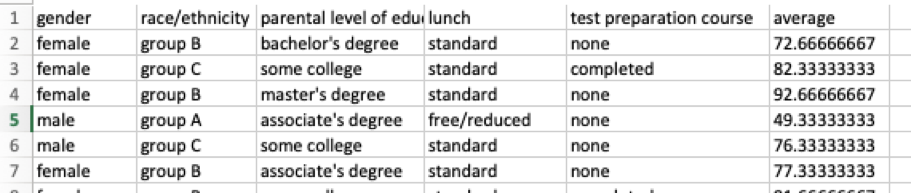
\includegraphics[scale=1]{src_img/StudentsPerformanceDataSetModif.png}
    \caption{Jeu de donnée final}
    \label{studentsPerformanceDataSetModif}
\end{figure}
Une fois notre modèle entraîné à prédire la moyenne potentielle d'un étudiant à partir de ces caractéristiques, on pourrai imaginer l'utiliser pour le recrutement universitaire. Mais (en dépit du fait que ces caractéristiques ne sont pas très pertinentes) notre modèle de recrutement est-il réellement fiable ? Pourrait-il être discriminant pour certaines ethnies ou pour un certain sexe ? Nous allons essayer de le découvrir en comprenant comment les caractéristiques d'entrée influent sur notre prédiction.

\subsection{Création du modèle prédictif}
La première étape sera donc de créer un modèle prédictif et de l'entraîner sur notre jeu de données. Pour ce faire, nous avons utilisé l'algorithme des forêts d'arbres décisionnels (random forest) qui fait partie de la famille des ensembles d'arbres vu dans l'état de l'art partie 2.2.3. Cet algorithme reposant sur l'apprentissage par arbre de décision consiste à effectuer un apprentissage en parallèle sur de multiples arbres de décision construits aléatoirement et entraînés sur des sous-ensembles de données différentes selon le principe du bagging. Le baggin consiste à réduire la variance d'un arbre de décision afin de palier à son instabilité. Les prédictions de tous ces arbres sont ensuite moyennées afin de nous donner un résultat.\par
Afin de créer notre modèle, nous allons utiliser une bibliothèque Python destinée à l'apprentissage automatique appelée Scikit-learn (sklearn)\cite{sklearnDepot}. Cette bibliothèque a été initiée en 2007 par David Cournapeau en tant que projet Google Summer of Code qui est un programme organisé par l'entreprise Google où des étudiants travaillent pendant l'été sur un projet pour lequel l'étudiant a postulé. Open source et comptant de nombreux collaborateurs, cette bibliothèque mettant à notre disposition une multitude d'outils pour le machine learning est devenue la référence dans son domaine notamment grâce à sa complétude et sa simplicité d'utilisation.\par
Afin d'être adapté à notre modèle, notre jeu de données a dû être encodé en créant une colonne par variables dans le but de n'avoir que des entrées numériques, par exemple la colonne "gender" devient deux colonnes "female" et "male" prenant 0 ou 1 comme valeur. Pour notre jeu de données, nous passons donc de cinq colonnes d'entrée à dix-sept colonnes qui sont : \medbreak
['x0\_female' 'x0\_male' 'x1\_group A' 'x1\_group B' 'x1\_group C' 'x1\_group D' 'x1\_group E' "x2\_associate's degree" "x2\_bachelor's degree" 'x2\_high school' "x2\_master's degree" 'x2\_some college' 'x2\_some high school' 'x3\_free/reduced' 'x3\_standard' 'x4\_completed' 'x4\_none']\medbreak
Où "x0" correspond à la transformation de la première colonne, "x1" à la transformation de la deuxième colonne et ainsi de suite.

\subsection{Explication de notre prédiction}
Notre modèle étant prêt, nous allons pouvoir nous demander s'il n'a pas été biaisé involontairement par notre jeu de données. Pour ce faire, nous allons utiliser un outil d'interprétation présenté dans notre état de l'art : SHAP, à l'aide de la librairie python SHAP vu dans notre état de l'art. La première chose à faire est de déterminer la valeur de Shapley de notre modèle, la librairie SHAP met à notre disposition une fonction prenant en paramètre notre modèle ainsi que nos données d'entraînement. Comme décrit dans l'état de l'art partie 2.3.2, cette fonction va sonder notre modèle de multiple fois en faisant varier les données d'entrées afin de déterminer l'impact de ces données sur notre prédiction.\par
Une fois notre valeur de Shapley obtenue, nous pouvons afficher différent graphique afin de mieux comprendre les raisons de nos prédictions. La figure \ref{shapPlotBar} est un graphique généré par SHAP fournissant une explication globale de notre modèle de type importance des variables (features importance). L’importance des variables est calculée en moyennant la valeur absolue des valeurs de Shapley de chaque variable pour chaque exemple de notre jeu de données.

On voit donc sur notre graphique que la non-préparation aux tests et qu'un régime alimentaire équilibré sont les deux entrées aillent le plus d'impact sur notre prédiction, mais nous ne sommes pour le moment pas en mesure de savoir si cet impact est positif ou négatif.

\begin{figure}[h]
    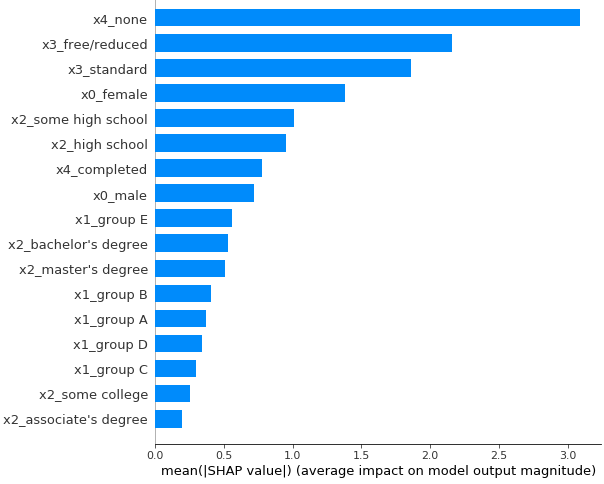
\includegraphics[scale=0.6]{src_img/shapPlotBar.png}
    \caption{Importance des variables d'entrées dans notre prédiction}
    \label{shapPlotBar}
\end{figure}
Afin d'entrer plus dans le détail, SHAP nous offre d'autres graphiques comme par exemple la figure \ref{shapPlotDetail}. Sur ce graphique, chaque point représente une valeur de Shapley pour la variable pour chacune des instances. Les points rouges représentent un impact positif sur notre prédiction et les points bleu représentent un impact négatif. Nos données d'entrée étant constituées de valeurs binaires, ce graphique se lis de cette manière : si la valeur est positive et que la couleur est bleu alors la variable a un impact négatif sur notre valeur de sortie et inversement pour la couleur rouge. Par exemple la non-préparation au test et un régime alimentaire équilibré ont une influence négative sur notre moyenne. On peut aussi voir qu'être une femme a un impact positif alors qu'être un homme a un impact négatif. L’ethnie de type D sera aussi favorisée. Ces résultats laissent penser qu'utiliser ce modèle pour le recrutement universitaire aura un effet discriminatoire pour les hommes qui seront défavorisés, ce qui ressemble à l’IA d’Amazon évoquée précédemment.
\begin{figure}[h]
    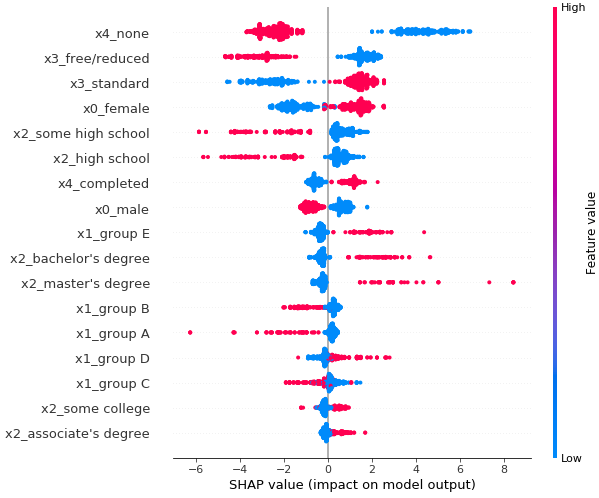
\includegraphics[scale=0.6]{src_img/shapPlotDetail.png}
    \caption{Détail de l'explication de l'importance des variables}
    \label{shapPlotDetail}
\end{figure}
Il nous est aussi possible de fournir une interprétation local c'est-à-dire de voir pourquoi notre boite noire a donnée un tel résultat pour une instance précise. La figure \ref{shapPlotLocal} nous montre un exemple d'interprétation local. On vois que pour cette instance notre modèle a estimé que l'étudiant aurai 60.62 de moyenne. Comme pour l'exemple précédent, les variables aillant un impact positif sont affichées en rouge et celles ayant un impact négatif sont affichées en bleu. On voit donc que pour cette instance l'entraînement à l'épreuve, le régime alimentaire et le sexe influence négativement notre moyenne alors que le niveau d’éducation des parents a une influence positive.
\begin{figure}[h]
    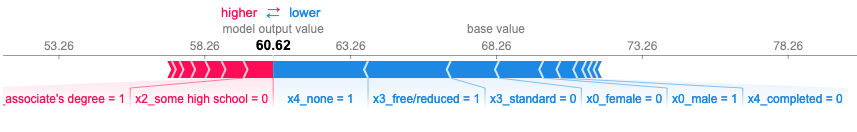
\includegraphics[scale=0.5]{src_img/shapPlotLocal.png}
    \caption{Explication de la prédiction pour une instance précise}
    \label{shapPlotLocal}
\end{figure}

\subsection{Bilan}
 Après l'inspection de notre modèle, nous avons pu voir qu'il jugeait les femmes plus performantes que les hommes et que son utilisation dans le recrutement universitaire aurai eut un impact discriminant sur les étudiants postulant. L'utilisation d'une méthode d'interprétabilité sur notre boite noire nous a donc permis de mettre en évidence un biais de discrimination présent dans notre jeu de donnée. Bien sûr, notre exemple étant trivial on aurai pu directement se rendre compte que les caractéristiques d'entrées n'étaient pas réellement pertinentes pour prédire la moyenne d'un étudiant.\par
 Nous pouvons donc dire que qu'il est important de vérifier la pertinence des entrées de notre modèle, aussi utiliser un algorithme permettant que comprendre la logique interne de notre boite noire est important afin d'éviter tous problèmes.

\section{Améliorer la fiabilité}
L'intelligence artificielle pose aussi des problèmes de fiabilités, notamment dans le domaine médical. Afin de savoir si rendre un modèle interprétable permettrai d'améliorer sa fiabilité et de vérifier s'il se base sur les bons éléments pour donner ses prédictions, nous allons appliquer l'algorithme LIME vu dans l'état de l'art à un modèle issu du monde médical.

\subsection{Le jeu de données}
Pour cette expérimentation, nous allons utiliser un jeu de données contenant des images de radiographies. Le but sera de créer un modèle permettant de détecter si le patient de la radiographie est atteint de pneumonie. Ce jeu de données disponible ici \cite{kagglePneumonia} est visible sur la Figure \ref{pneumoniaImg} :
\begin{figure}[h]
    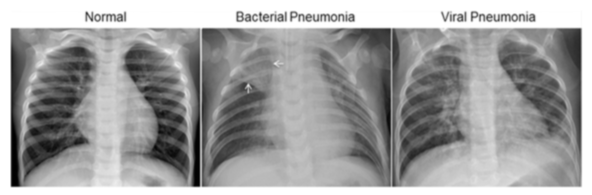
\includegraphics[scale=0.7]{src_img/pneumoniaImg.png}
    \caption{Exemple d'images présentes dans le jeu de donnée de pneumonie}
    \label{pneumoniaImg}
\end{figure}
Le jeu de données contient donc des radiographies de cages thoraciques saines ou malade. Dans la partie suivante, nous allons donc créer un modèle prenant en entrée une radiographie et nous donnant une prédiction sur l'état de santé du patient.

\subsection{Création du modèle prédictif}
Afin de prédire si la radiographie présente une pneumonie ou pas, nous allons créer un réseau de réseau de neurones à convolution. Un réseau de neurones à convolution (Convolutional Neural Networks). Cette algorithme, faisant partie de la famille des réseaux de neurones profond vu dans l'état de l'art partie 2.2.3, va ajouter des filtres et des couches à notre image d'entrée afin de pouvoir détecter plus de patterns que le ferai un réseau de neurones classique. Le code de ce modèle est disponible sur mon GitHub \cite{pneumoniaDepot} et a été créé en Python à l'aide de TensorFlow 2.0.\par
TensorFlow\cite{tensorflowDepot} est un outil d'apprentissage automatique initié par Google en 2011 devenu en 2015 open source et comptant de nombreux collaborateurs. TensorFlow met à notre disposition une API stable pour les langages Python et C++, et est devenu l'un des outils les plus utilisés en matière d'intelligence artificielle notamment pour la création d'architecture de réseau de neurones artificiels.

\subsection{Explication de notre prédiction}
Notre modèle prêt, nous allons utiliser l'algorithme de LIME présenté dans notre état de l'art afin de vérifier la fiabilité de notre modèle. Dans cette partie, nous n'utiliserons pas la librairie LIME afin de pouvoir entrer plus dans le détail du fonctionnement de cette algorithme et de mieux le comprendre. Le code correspondant à l'implémentions de LIME est disponible sur mon GitHub \cite{limeMyDepot} et suit, entre autre, le tutoriel de "Towards Data Science" \cite{limeTuto}. L'explication sera locale et effectuée sur une seule image. Pour rappel,  l’idée de LIME est de sonder la boite noire autant de fois que nécessaire avec différentes versions de notre image d'entrée qui aura subi de multiples perturbations.\par
La première étape consiste donc à créer des perturbations pour notre image. Pour ce faire, nous allons utiliser la librairie Skimage afin de générer 75 perturbations de notre image. La figure \ref{limePerturbSchema} montre le squelette de perturbation de notre image, chaque zone sera cachée ou affichée comme le montre la figure \ref{limePerturbExemple}.\par
\begin{figure}[h]
    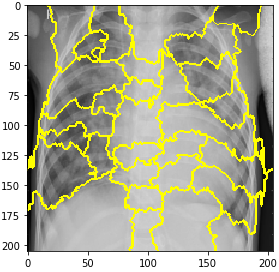
\includegraphics[scale=0.6]{src_img/limePerturbSchema.png}
    \caption{Zones de perturbation}
    \label{limePerturbSchema}
\end{figure}

\begin{figure}[h]
    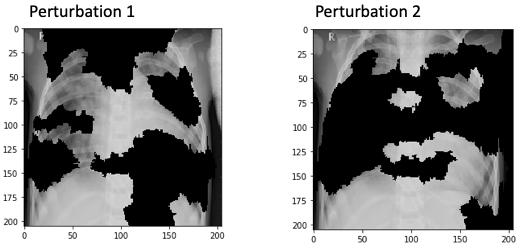
\includegraphics[scale=0.7]{src_img/limePerturbations.png}
    \caption{Exemple de perturbations générées}
    \label{limePerturbExemple}
\end{figure}

La seconde étape consiste à utiliser notre modèle afin d'effectuer une prédiction pour l'ensemble des perturbations générées. La prédiction ne doit pas nous donner le résultat, mais sa probabilité. Pour notre exemple la prédiction ne renverra donc pas "pneumonie", mais un tableau de deux valeurs avec la probabilité d'avoir que les poumons soient sains ou non "[0.23, 0.77]".\par
Une fois nos prédictions faites, nous allons évaluer la distance entre chaque prédiction et notre image de base. La distance correspond aux nombre de zones du squelette de perturbation de la figure \ref{limePerturbSchema} cachées. L'image de base aillant toutes les zones de perturbation visible.\par
Pour finir, nous créons un modèle linéaire que nous entraînons avec les informations obtenues dans les étapes précédentes afin d'obtenir un coefficient pour chacune des zones de perturbations représentant l'importance de la zone pour notre prédiction. Il ne nous reste donc plus qu'à trier ces coefficient afin d'afficher les quatre plus élevés. Pour notre exemple nous obtenons le résultat présenté en figure \ref{limeFinalExplain} sur l'image de gauche.

Afin d'y voir plus clair, nous pouvons superposer l'image obtenue avec l'image de base afin de voir la zone du poumon touchée par la pneumonie selon notre réseau de neurones comme le montre la figure \ref{limeFinalExplain} sur l'image de droite.

\begin{figure}[h]
    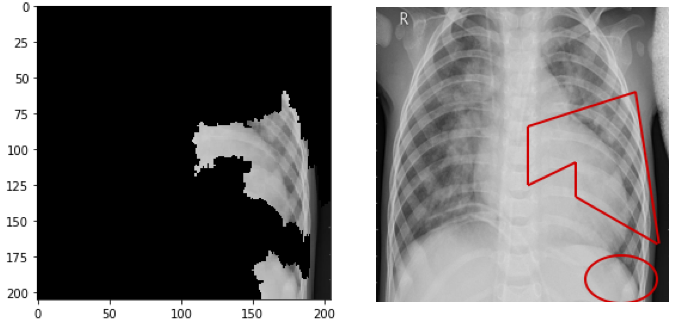
\includegraphics[scale=0.58]{src_img/limeFinalExplainMerge.png}
    \caption{À gauche : Zones de perturbations avec les coefficients les plus élevés
    À droite : Explication de la prédiction de pneumonie par LIME}
    \label{limeFinalExplain}
\end{figure}
\subsection{Bilan}
L'utilisation de l'outil d'interprétabilité nous a donc bien permit de déterminer quelles zones de notre image sont déterminantes pour notre prédiction. Dans notre exemple l'explication apporte un plus à la simple prédiction "pneumonie", car elle montre la zone la plus touchée par la maladie.\par
Accompagner chaque prédiction avec son explication serait un grand plus et améliorer grandement la fiabilité de nos modèles. Aussi, cela permettrai d'augmenter la confiance de la population à l'égard de ces technologies. Bien-sûr le but n'est pas de faire vérifier chaque prédiction par un médecin, cela serai contre-productif et l'IA permettant de faire gagner du temps aux médecins serait inutile. L'idée serait d'utiliser ces prédictions pendant les phases de développement et de test de notre IA afin de vérifier qu'elle évolue dans le bon sens et qu'elle détecte bien les pneumonies et pas autre chose.

%\chapter*{Conclusion}
%\addcontentsline{toc}{chapter}{Conclusion}
%\markboth{Conclusion}{Conclusion}
%\label{sec:conclusion}

\chapter{Ouverture}

\paragraph{}En plus de résoudre les questions d'éthique, de fiabilité et de performance vue dans ce mémoire, l'interprétabilité et l'explicabilité des modèles prédictifs nous permettrait d'ouvrir de nouvelles portes. L'essor de l'intelligence artificielle et, en parallèle, son explication permet d'introduire un nouveau concept que j'ai appelé "L'intelligence artificielle comme compréhension du monde". L'idée est de détourner l'IA de sa fonction de prédiction de phénomènes pour lui donner une toute autre fonction qui serait la compréhension de phénomène. Le principe est de prendre un phénomène que nous ne comprenons pas entièrement, de réussir à le prédire à l'aide d'un modèle, puis d'expliquer ce modèle avec les algorithmes d'interprétabilité afin de comprendre ce qui l'amène à donner ces prévisions et donc de mieux comprendre le phénomène de base.

\paragraph{}Prenons un exemple trivial, imaginons que nous ne comprenons pas comment les éclairs se forment dans les nuages. Dans un premier temps, nous commencerons par récolter une multitude de données météorologiques et autre. Puis nous créons un modèle prenant ces données en entrée et capable de prédire la formation d'éclairs. La dernière étape consiste donc à expliquer notre modèle afin de comprendre quels facteurs entrent en jeu dans la formation des éclairs, ainsi que l'importance de ces facteurs (type de nuage, répartition des charges positives et négatives...).

\paragraph{}Ce concept appliqué dans les domaines de l'infiniment petit ou de l'infiniment grand par exemple, pourrait nous aider à mieux comprendre certains phénomènes encore aujourd'hui non-expliqué.

\newpage
\begin{appendices}

\section{Revue des méthodes explicatives}
\begin{figure}[h]
\centering
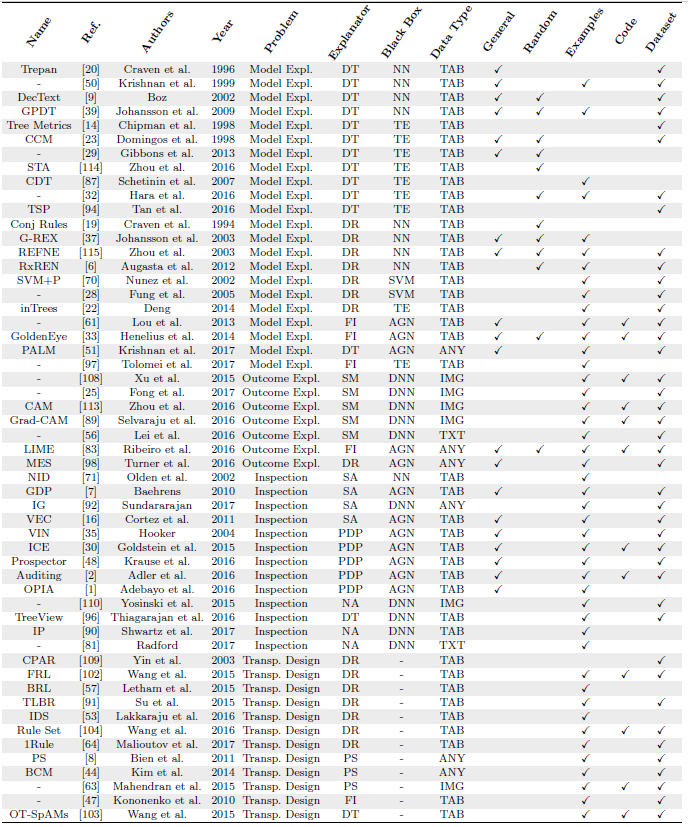
\includegraphics[scale=0.97]{src_img/tabSummary.PNG}
\caption{Tableau résumant l'ensemble des méthodes expliquant les boites noires présent dans la littérature. Description en annexe 2. Tiré de \cite{surveyExplaining}}
\label{tabSummary}
\end{figure}

\newpage

\section{Description des méthodes explicatives}
\begin{figure}[h]
\centering
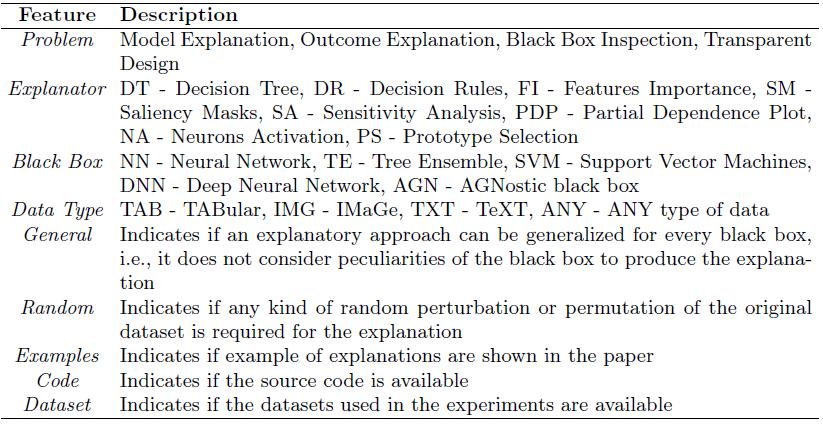
\includegraphics[scale=1.01]{src_img/descSummary.PNG}
\caption{Description du tableau présent en annexe 1. Tiré de \cite{surveyExplaining}}
\label{descSummary}
\end{figure}

\end{appendices}


\newpage
%\nocite{SpaceXFirstISS, IFPI2011Report, SpotifyBloomberg, SpotifyNewYorker}

\printbibliography[title={Bibliographie},nottype=online]

\printbibliography[title={Webographie},type=online]

\newpage
\listoffigures
\chapter*{Liste des Acronymes}
\begin{acronym}[DNN] % Give the longest acronym here
\acro{IA}{\emph{Intelligence artificielle}}
\acro{NN}{\emph{Réseau de neurones (Neuronal Network)}}
\acro{DNN}{\emph{Réseau de neurones profond (Deep Neuronal Network)}}

\end{acronym}

\newpage
\thispagestyle{empty}
\vspace*{\fill}
\begin{center}
  Université Paris-Nanterre\\
  200 Avenue de la République\\
  92000 Nanterre
\end{center}
\vspace*{\fill}

\end{document}